%! Mode:: "TeX:UTF-8"
%! TEX program = xelatex
\PassOptionsToPackage{quiet}{xeCJK}
\documentclass[withoutpreface,bwprint]{cumcmthesis}
\usepackage{etoolbox}
\BeforeBeginEnvironment{tabular}{\zihao{-5}}
\usepackage[numbers,sort&compress]{natbib}  % 文献管理宏包
\usepackage[framemethod=TikZ]{mdframed}  % 框架宏包
\usepackage{url}  % 网页链接宏包
\usepackage{subcaption}  % 子图宏包
\allowdisplaybreaks % 允许在align环境中分页
\newcolumntype{C}{>{\centering\arraybackslash}X}
\newcolumntype{R}{>{\raggedleft\arraybackslash}X}
\newcolumntype{L}{>{\raggedright\arraybackslash}X}

\title{基于非线性规划对扶壁式挡土墙稳定性最优化设计模型}  % 论文标题
\tihao{}  % 题号
\baominghao{}  % 报名号
\schoolname{}  % 学校
\membera{}  % 队员a
\memberb{}  % 队员b
\memberc{}  % 队员c
\supervisor{}  % 指导老师
\yearinput{}
\monthinput{}
\dayinput{}

%%%%%%%%%%%%%%%%%%%%%%%%%%%%%%%%%%%%%%%%%%%%%%%%%%%%%%%%%%%%%
%% 正文
\begin{document}

\maketitle
\begin{abstract}%摘要
在高速公路山体滑坡治理中,挡土墙的防护起到了至关重要的作用。
作为保护高速公路免受山体滑坡影响的最后一道屏障,研究如何利用数学模型提高挡土墙稳定性
使得高速公路的安全性大大提升,是我们亟待解决的问题。
\par
\textbf{对于问题一,}
首先,对\textbf{几何参数}、\textbf{材料参数}和\textbf{荷载参数},分别确定不同参数对单段扶壁式挡土墙的约束。
其次,通过建立\textbf{抗倾覆稳定性模型和抗滑移稳定性模型},采用\textbf{库仑土压力理论}计算主动土和被动土压力值的计算。
在抗倾覆安全系数和抗滑移安全系数求解后,最终通过\textbf{偏导}的方式,可以得到稳定性和内摩擦角$\varphi$、墙面板与墙址板的夹角$\alpha$正相关。


\par
\textbf{对于问题二,}
首先,针对单段扶壁式挡土墙的\textbf{几何参数、材料参数和荷载参数},
分别确定了不同的约束条件:几何参数方面,
明确了底桩半径\(L\)、深度\(D\)、
间隔\(L_2\)等新增参数的范围;
材料参数上,明确了钢筋屈服强度、混凝土轴心抗拉强度等关键指标;
荷载参数则新增了底柱对土层的侧向摩擦力\(F_p\),
并建立了其与单位摩擦力\(T_f\)的关系。
\textbf{稳定性随$\alpha$(墙面板与墙趾板的夹角)的增大而单调递增,随$\beta$(墙面板与墙踵板的夹角)的增大而单调递减}。
最终通过建立\textbf{基于非线性规划的钢筋位置稳定性最优化设计模型}得出,当钢筋位置\textbf{在($x$,$y$)=(0.3000,0.2434), 并且深度为 5.6米,结果最优}。

\par
\textbf{对于问题三,}
在问题一、二模型基础上,新增加有关积水对挡土墙影响因素。
在建模过程中,重点考虑了浮力对土体重度影响,修正了主动土压力和被动土压力在浮力作用下的大小,
利用\textbf{水压力分布公式},我们最终得到了\textbf{基于非线性规划的泄水孔位置及数量稳定性最优化设计模型}。
在模型求解中,我们通过 \textbf{COBYLA 算法}简化步骤,最终得到\textbf{泄水孔半径为0.142米,总共有4层,其中每层泄水孔坐标分别为其坐标分别为(0.44,1.25/1.94/3.44/4.94),(4.15,1.25/1.94/3.44/4.94),(7.05,1.25/1.94/3.44/4.94),(9.95,1.25/1.94/3.44/4.94),单位为米}。
\par
% \textbf{对于问题四,}
\keywords{库仑土压力理论\quad  COBYLA 算法\quad  水压力分布 \quad 非线性规划}
% 最后,
\end{abstract}
%%%%%%%%%%%%%%%%%%%%%%%%%%%%%%%%%%%%%%%%%%%%%%%%%%%%%%%%%%%%% 

% \tableofcontents  % 目录
% \newpage

%%%%%%%%%%%%%%%%%%%%%%%%%%%%%%%%%%%%%%%%%%%%%%%%%%%%%%%%%%%%%  
\section{问题重述}
\subsection{问题背景}
近年来。随着极端天气、人类活动及众多因素的影响下,高速公路旁的山体滑坡现象频发。
加强对高速公路高边山坡的滑坡问题的重视,对高速公路的建设有着极大正向影响,可以在一定程度上减少相关悲剧发生。
\par
山体滑坡的物质基础是因其结构松散的特性,在强降雨情况下容易发生变化。
而其他内在因素则有包括地貌、地震、河流及相关的人类活动。
为防治高速公路的滑坡,应采取多方面综合山体滑坡防治体系。一方面应保护并利用相关的地质环境,另一方面需调查并研究,
采用相应处理的技术措施以避免大规模的滑坡。\upcite{SJCZ201701069}
\par
在防治高速公路山体滑坡的体系中,挡土墙以其独特的结构功能与技术优势,占据着不可替代的核心地位,成为保障高速公路边坡稳定的重要工程措施。
其中,国内外关于扶壁式挡土墙的研究较少,亟须对高速公路组合扶壁式挡土墙力学特性开展研究。\upcite{JZGC202506001}
\par
因此,针对高速公路的滑坡问题,对扶壁式挡土墙相关参数的研究及处理,是保障人民生命及财产安全的重要手段。
%%%%%%%%%%%%%%%%%%%%%%%%%%%%%%%%%%%%%%%%%%%%%%%%%%%%%%%%%%%%% 

\subsection{问题要求}

\textbf{问题1}  
在不考虑挡土墙的底桩并且满足挡土墙不能滑动、倾倒且有一定的强度与抗压力情况下,
确定单段扶壁式挡土墙的相关参数,并且建立数学模型来分析相关参数和挡土墙稳定性的影响。
其中,尤其要考虑到内摩擦角以及墙面板、墙趾板之间的夹角与稳定性的关系。
\par
\textbf{问题2}  
在问题一的模型上,考虑挡土墙的底桩对不同参数的影响。并且分析稳定性和墙面板、墙趾板角度和墙面板、墙踵板角度的关系。
同时,在考虑多段挡板土墙同时施工情况下,通过设计拉筋位置来使得稳定性最优化。
\par
\textbf{问题3} 
由于暴雨因素影响,挡土墙的透水性容易变差进而导致总体压力不足使得挡土墙倾覆。
因此需要考虑在挡土墙中,如何设置泄水孔位置及尺寸来增强扶壁式挡土墙稳定性。
% \textbf{问题4}  

%%%%%%%%%%%%%%%%%%%%%%%%%%%%%%%%%%%%%%%%%%%%%%%%%%%%%%%%%%%%% 

\section{问题分析}
\subsection{问题一分析}
对于问题一,我们在基于题目及相关资料上,认为相关重要参数应该和几何参数、材料参数和荷载参数有关联。
在此基础上,决定建立抗倾覆稳定性模型和抗滑移稳定性模型,对主动土和被动土拉力进行理论上求解。
在求解过程中,通过推导抗倾覆安全系数和抗滑移安全系数,最终利用偏导得到答案。

\subsection{问题二分析}	
对于问题二,在问题一模型基础上,新增底桩相关参数并明确其约束条件,
包括底桩半径、深度、间隔等几何参数范围,钢筋和混凝土的材料强度指标,
以及底桩侧向摩擦力与单位摩擦力的关系。
核心在于分析稳定性与墙面板和墙趾板夹角(\(\alpha\))、墙面板与墙踵板夹角(\(\beta\))的关系,
通过推导含底桩参数的抗倾覆和抗滑移安全系数模型,得出稳定性随\(\alpha\)增大而单调递增、随\(\beta\)增大而单调递减的规律。
同时,针对多段挡土墙施工,建立基于非线性规划的钢筋位置最优化模型,综合考虑钢筋的位置约束、锚固长度等条件,
求解得出最优钢筋位置和底桩深度,以实现稳定性最大化。

\subsection{问题三分析}
对于问题三,在问题一、二模型基础上,重点考虑积水对挡土墙的影响,
需修正浮力作用下的土体重度,进而调整主动土压力和被动土压力计算。通过建立水压力分布公式,
量化泄水孔对水压力的折减效果,其中泄水孔层数根据墙高设定上限(本题取 4 层,间距 1.5 米),
并明确单孔排水效率系数与孔面积、间距等参数的关系。最终构建基于非线性规划的泄水孔位置及数量最优化模型,
以抗倾覆和抗滑移安全系数为目标函数,结合泄水孔位置范围、半径等约束条件,求解得出最优泄水孔参数,
最大限度降低积水对稳定性的不利影响。


%%%%%%%%%%%%%%%%%%%%%%%%%%%%%%%%%%%%%%%%%%%%%%%%%%%%%%%%%%%%% 

\section{模型假设}

为简化问题,本文做出以下假设:

\begin{itemize}[itemindent=2em]
\item 假设单个扶壁式挡土墙扶肋为3个;
\item 假设挡土墙两侧土水平最高与墙面板持平;
\item 假设工程使用的C35混凝土和H2B400钢筋;
\item 假设填土为均质、各向同性的无粘性土,忽略粘聚力;
\item 假设挡土墙为刚性体,不考虑自身变形对稳定性的影响;
\item 假设底桩与土体之间的摩擦力沿深度线性分布,单位摩擦力\(\tau\)为常数;
\item 假设钢筋为理想弹塑性材料,忽略应力松弛和徐变效应;
\item 假设积水对挡土墙的作用简化为静水压力,采用三角形分布模型;
\item 假设泄水孔排水效率系数\(\eta\)为常数,不考虑孔道堵塞或渗透系数变化。
\end{itemize}

%%%%%%%%%%%%%%%%%%%%%%%%%%%%%%%%%%%%%%%%%%%%%%%%%%%%%%%%%%%%% 


\section{符号说明}
\begin{table}[H]
\centering
\begin{tabularx}{\textwidth}{CCC}  % 三列均居中对齐
\toprule
符号    & 说明    & 单位 \\
\midrule
$H     $& 墙高 & $m$ \\
$t     $& 扶肋厚度 & $m$ \\
$B_1   $& 墙面板顶宽 & $m$ \\
$B_2   $& 墙趾板宽度 & $m$ \\
$L     $& 扶肋间距 & $m$ \\
$E_a   $& 主动土压力 & $N$ \\
$E_b   $& 被动土压力 & $N$ \\
$\gamma_1     $& 挡土墙材料的重度 & $kg/m^3$ \\
$\gamma_2     $& 土体的重度 & $kg/m^3$ \\
$G     $& 挡土墙自重 & $kg$ \\
$M_t     $& 倾覆力矩 & $N\cdot m$ \\
$M_r     $& 抗倾覆力矩 & $N\cdot m$ \\
$F_s     $& 滑动力 & $N$ \\
$F_r     $& 抗滑力 & $N$ \\
%\midrule  % 用分隔线区分有单位和无单位的符号
$\alpha$& 墙面板与墙趾板间的夹角 & $/$ \\
$\beta $& 墙面板与墙趾板间的夹角 & $/$ \\
$K_a     $& 主动土压力系数 & $/$ \\
$K_b     $& 被动土压力系数 & $/$ \\
$K_t     $& 抗倾覆安全系数 & $/$ \\
$K_s     $& 抗滑安全系数 & $/$ \\
\bottomrule
\end{tabularx}
\label{tab:符号说明}
\end{table}


%%%%%%%%%%%%%%%%%%%%%%%%%%%%%%%%%%%%%%%%%%%%%%%%%%%%%%%%%%%%% 

\section{问题一的模型的建立和求解}
\subsection{重要参数的确定}
为方便后续问题求解,我们将题目中涉及到挡土墙的有关参数进行了提取,并对不同参数进行了约束。
\par
%%%%%%%%%%%%%%%%%%%%%%%%%%%%%%%%%%%%%%%%%%%%%%%%%%%%%%%%%%%%%%%%%%%%%
\subsubsection{几何参数的确定}
我们规定了以下重要几何参数:$H$表示墙高,其约束为不超过30m;$L$表示扶肋间距,约束条件为不超过墙高的一半;
$t$表示扶肋厚度,约束条件为$\frac{L}{10}$到$\frac{L}{4}$,且大于0.3米;
$B_1$表示墙面板顶宽,约束条件为$\frac{H}{4}$到$\frac{H}{2}$,且大于0.5米;
$B_2$表示墙址板宽度,约束条件为$\frac{H}{20}$到$\frac{H}{5}$,且大于0.3米;
$\alpha$ 表示墙面板与墙趾板间的夹角;
$\beta$ 表示墙面板与墙踵板的夹角。
同时为方便说明,我们将墙面板设定为$b$,上部分规定为$b_1$,,墙面板下方的左侧为$b_{21}$,右侧为$b_{22}$。
下图为墙面板和墙趾板的主视图和侧视图及相关参数:

    \begin{figure}[H]
    \centering
    \subcaptionbox{墙面板和墙趾板的主视图\label{fig:墙面板和墙趾板的主视图}}
    {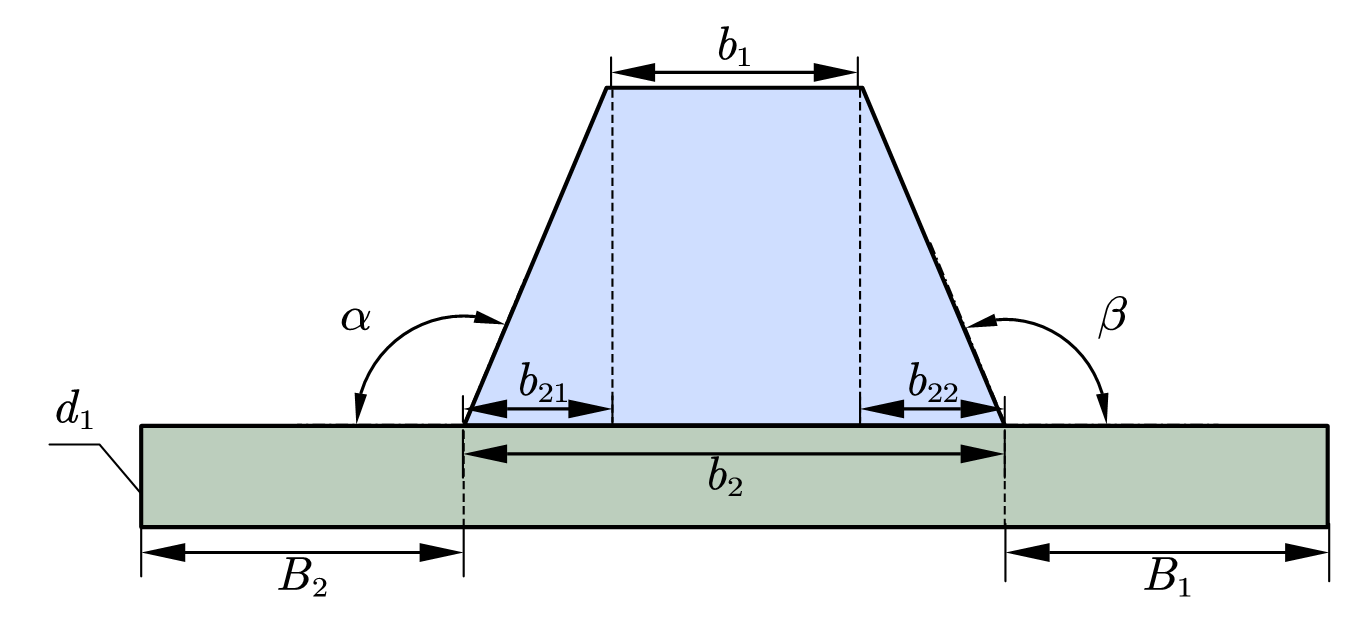
\includegraphics[width=.4\textwidth]{坐标1.png}}
    \subcaptionbox{墙面板和墙趾板的侧视图\label{fig:墙面板和墙趾板的侧视图}}
    {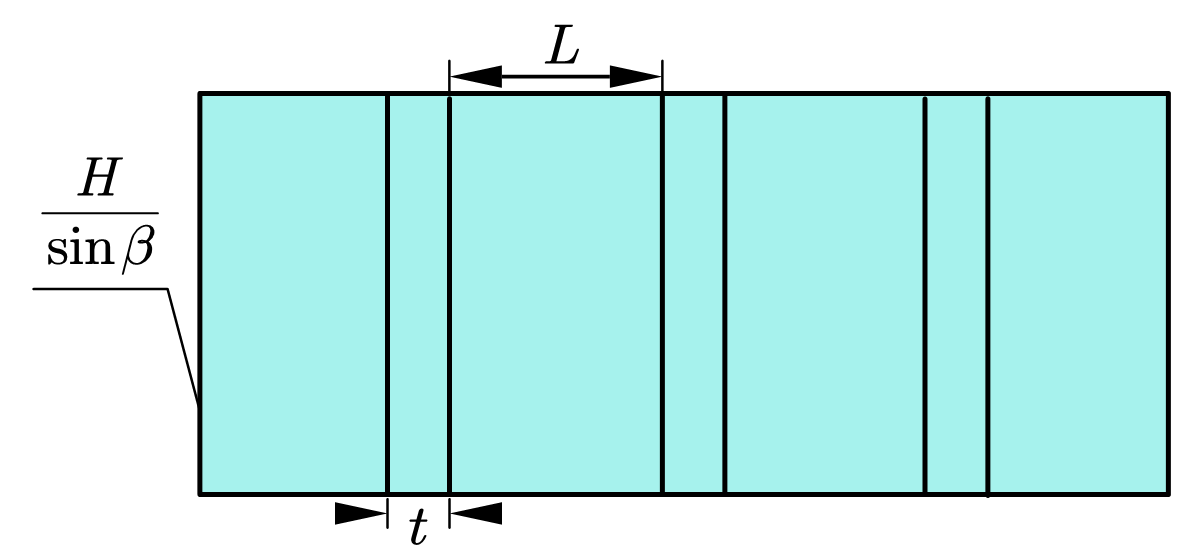
\includegraphics[width=.4\textwidth]{坐标2.png}}
    \caption{墙面板和墙趾板主视图和侧视图}\label{fig:墙面板和墙趾板主视图和侧视图}
    \end{figure} 

同时,我们将上述几何约束条件数学化,可以得到以下约束条件:
\begin{equation}
    s.t.    
    \begin{aligned}
        \begin{cases}
            H\leq30 \\
            L\leq\frac{H}{2} \\
            t\in[\frac{L}{10},\frac{L}{4}],t\geq0.3 \\
            b=k_{1}(B_{1}+B_{2}+b_{2})=k_{3}L \\
            b_{1}\geq0.2 \\
            B_{1}\in[\frac{H}{4},\frac{H}{2}],B_{2}\geq0.5 \\
            B_{2}\in[\frac{H}{20},\frac{H}{5}],B_{2}\geq0.3 \\
            b_{2}=b_{21}+b_{1}+b_{22} \\
            4L+3t\leq40 \\
            tan\alpha=-\frac{H}{b_{21}},tan\beta=-\frac{H}{b_{22} }
        \end{cases}
    \end{aligned}
\end{equation}
上述公式中,我们约定$\alpha$、$\beta$是墙面板与墙趾板、墙踵板分别向外部方向的夹角。

\subsubsection{材料和荷载参数设定}
\begin{itemize}
    \item \textbf{材料参数}
\par
    建筑结构的稳定性不仅在于其框架结构的科学性,原材料改良加固也可以有效提高填充材料的紧密性,避免建筑的开裂、收缩等问题。\upcite{YSLX202306018}
    因此我们考虑到墙体、土体等材料因素。
    我们规定了以下参数:
    $\gamma_1$ 表示挡土墙材料的重度;$\gamma_2$ 表示土体的重度;
    $\varphi$表示土体的内摩擦角。
    在查阅相关文献后\upcite{2019Seismic},我们确定了$\gamma_1$=24,$\gamma_2$=18。
    \item \textbf{荷载参数}
\par
    同时,考虑到后续墙体的受力分析,我们认为需要将土分成墙前和墙后两个方面考虑。
    其中,$E_a$表示墙后土体产生的主动土压力,$E_b$表示墙前土体产生的主动土压力,$G$表示挡土墙自重。
\end{itemize}

\subsubsection{强度参数设定}
为了提升模型的准确度,满足题目中挡土墙有足够的强度和承载力,我们设定了强度参数加以约束:

\textbf{最大弯矩:}
墙面板承受主动土压力产生的均布荷载,按简支梁计算最大弯矩,再验算弯曲应力是否小于混凝土轴心抗拉强度设计值 $f_t $(因面板受拉区控制设计)。
其中最大弯矩计算公式为:

    \begin{equation}
        M_{\text{max}} = \frac{q \cdot L^2}{8}
    \end{equation}
    \par
其中,均布荷载$q$由填土主动土压力产生,其计算公式基于土力学中主动土压力的基本原理,具体为:
    \begin{equation}
        q = \gamma \cdot h \cdot K_a
    \end{equation}
    \par
其中,$\gamma$ 为填土重度(文中取值 $18 \, \text{kN/m}^3$);$h$ 为计算点处的填土高度(对于均布荷载简化计算,此处取墙高范围内的平均或特征高度,结合文中参数推导得出对应值);$K_a$ 为主动土压力系数,由填土内摩擦角 $\varphi$ 确定,公式为 $K_a = \tan^2\left(45^\circ - \frac{\varphi}{2}\right)$(文中 $\varphi = 35^\circ$,计算得 $K_a \approx 0.27$)。\par
通过上述参数代入,最终求得文中 $q = 45 \, \text{kN/m}$。
代入$L$ = 3m,可以得到$M_{\text{max}}$=50.625 $\, \text{kN·m}$。

\textbf{截面抵抗矩:}
我们约定$W$为截面抵抗矩:对于单位宽度面板(取扶肋间距 $L$为计算宽度),矩形截面抵抗矩公式为:

    \begin{equation}
        W = \frac{L \cdot b_1^2}{6}
    \end{equation}

其中 $b_1 = 0.3 \, \text{m}$ (面板厚度),代入得:
$W = \frac{3 \times 0.3^2}{6} = 0.045 \, \text{m}^3$

\textbf{截面抵抗矩:}我们约定 $W$为截面抵抗矩,对于单位宽度面板,矩形截面抵抗矩公式为:
    \begin{equation}
        W = \frac{L\cdot b_1^2}{6}
    \end{equation}

其中 $b_1 = 0.3 \, \text{m}$(面板厚度),代入得:
$W = \frac{3 \times 0.3^2}{6} = 0.045 \, \text{m}^3$
\par

\textbf{截面抵抗矩:}我们约定 $\sigma_{\text{弯}}$为弯曲应力,其公式为:
    \begin{equation}
        \sigma_{\text{弯}} = \frac{M_{\text{max}}}{W}
    \end{equation}


代入数据得:
$\sigma_{\text{弯}} = 1.125 \, \text{MPa} \leq f_t = 1.43 \, \text{MPa} $。可以看出满足以上约束条件。


\textbf{最大剪力:}我们约定最大剪力为$V_{\text{max}}$,则对应的公式为:
    \begin{equation}
        V_{\text{max}} = \frac{q \cdot }{2}    
    \end{equation}


代入 $q = 45 \, \text{kN/m}$、$L = 3 \, \text{m}$ 得:$V_{\text{max}} = \frac{45 \times 3}{2} = 67.5 \, \text{kN} $
\par
\textbf{剪应力:} 我们约定剪应力为$\tau$,矩形截面剪应力公式(取平均剪应力近似计算)为:
    \begin{equation}
        \tau = \frac{V_{\text{max}}}{A_f}
    \end{equation}

其中 $A_f = t \cdot H$ 为扶肋截面面积($t = 0.4 \, \text{m}$ 为扶肋厚度,$H = 8 \, \text{m}$ 为墙高)。  
代入数据得:$\tau \approx 21.09 \, \text{kPa} \leq f_t = 1430 \, \text{kPa} $。


\textbf{地基压应力:}
墙身自重与土压力合力对地基产生的最大压应力,需小于地基承载力特征值 $[p]$。
墙身自重 $G = 420 \, \text{kN}$,主动土压力合力 $E_a \approx 540 \, \text{kN}$(根据 $E_a = \frac{1}{2} \gamma H^2 K_a$,$K_a$ 为主动土压力系数,由 $\varphi = 35^\circ$ 计算得 $K_a \approx 0.27$)。
通过力矩平衡计算,合力作用点距墙趾距离 $e \leq B/6$($B = B_h + B_t = 3.7 \, \text{m}$ 为基底总宽),满足偏心距要求。
$p_{\text{max}}$:矩形基础偏心受压时最大压应力公式为:
    \begin{equation}
        p_{\text{max}} = \frac{G + E_{a,y}}{B} \left(1 + \frac{6e}{B}\right)
    \end{equation}


其中 $E_{a,y}$ 为土压力竖向分力(约 $80 \, \text{kN}$),代入数据得:$p_{\text{max}} \approx 190 \, \text{kPa} \leq [p] = 250 \, \text{kPa} $
%%%%%%%%%%%%%%%%%%%%%%%%%%%%%%%%%%%%%%%%%%%%%%%%%%%%%%%%%%%%%%%%%%%%%%%%%%%%%

\subsection{抗倾覆稳定性模型和抗滑移稳定性模型的建立}

\subsubsection{主动土、被动土压力的计算}

\textbf{Step1:主动土、被动土压力理论计算} 
\par
在对主动土、被动土压力的计算时,我们采用库仑土压力理论,分别对主动土和被动土压力讨论求解,具体公式如下:
    \begin{equation}
        \left\{
            \begin{aligned}
                E_a=\frac{1}{2} \gamma_2 H^2K_a\\
                E_b=\frac{1}{2} \gamma_2 H^2K_b
            \end{aligned}
        \right.
    \end{equation}
\par
    上式中,其中$K_a$为主动土压力系数,$K_b$为被动土压力系数,两者均与$\varphi$、$\alpha$及墙背摩擦角相关。

\textbf{Step2:主动土、被动土压力系数的推导} 
\par
    墙后土体对挡土墙的压力是导致滑移和倾覆的主要荷载,需用经典土压力理论计算主动土压力。
    我们考虑土体为无粘性土,可以得到主动土、被动土压力系数:
    \begin{equation}
            \left\{
            \begin{aligned}
                K_a=\frac{\cos^2(\varphi-(\beta-\frac{\pi}{2}))}{\cos^2(\beta-\frac{\pi}{2})\cdot\cos((\beta-\frac{\pi}{2})+\delta)\left[1+\sqrt{\frac{\sin(\varphi+\delta)\sin(\varphi-\beta_1)}{\cos((\beta-\frac{\pi}{2})+\delta)\cos((\beta-\frac{\pi}{2})-\beta_1)}}\right]^2}\\
                K_b=\frac{\cos^2(\varphi-(\alpha-\frac{\pi}{2}))}{\cos^2(\alpha-\frac{\pi}{2})\cdot\cos((\alpha-\frac{\pi}{2})+\delta)\left[1+\sqrt{\frac{\sin(\varphi+\delta)\sin(\varphi-\beta_1)}{\cos((\alpha-\frac{\pi}{2})+\delta)\cos((\alpha-\frac{\pi}{2})-\beta_1)}}\right]^2}
            \end{aligned}
            \right.
    \end{equation}
    
    上述公式中,其中:$\delta$ 为土与墙面板的摩擦角(我们土设定为混凝土,即$\delta = \dfrac{\varphi}{3}$),
    $\beta_1$为墙后填土表面倾角(我们假设水平时$\beta_1$=0)。
    \par

% \textbf{Step3:} 


\subsubsection{抗倾覆安全系数的求解}
抗倾覆安全系数求解公式如下:
    \begin{equation}
        K_t=\frac{M_r}{M_t}
    \end{equation}
    \par
其中:
\par
    \textbf{倾覆力矩$M_t$}:由主动土压力的水平分量产生,绕墙趾(墙址板前端点$O$)旋转,促使挡土墙倾倒;
 \par   
 \textbf{抗倾覆力矩$M_r$}:由挡土墙自重(墙面板、扶肋、墙址板、墙踵板的重力)、墙踵板上覆土的重力产生,阻碍倾倒。


\subsubsection{抗滑移安全系数的求解}
抗滑安全系数求解公式如下:
    \begin{equation}
        K_s=\frac{F_r}{F_s}
    \end{equation}
    \par
其中:
\par
\textbf{滑动力$F_s$:}主动土压力的水平分量,促使挡土墙沿地基表面滑动;
\par
\textbf{抗滑力$F_r$:}由挡土墙总自重$G$产生的摩擦力,以及墙址板上土体反力的垂直分量产生的附加摩擦力。

\subsection{模型求解}
\subsubsection{代入参数}
将上述各个参数代入到公式中,求解主动土、被动土压力,可得:
    \begin{equation}
        \begin{array}{l} 
        V=\frac{3B_1Ht}{2}+(B_1+B_2+b_2) (4l+3t)d_1+\frac{1}{2}(b_1+b_2)(4l+3t)H\\[0.2cm]
            \left\{
            \begin{aligned}
                &K_s=\frac{(\gamma_1 V+(4L+3t)E_{ay}+(4L+3t)E_{by})\mu +(4l+3t)E_{bx}}{E_{ax}} \\
               &K_t = \frac{G_{ax} + (4l + 3t)(E_{ay}X_{ay} + E_{by}X_{by})}{E_{ax}h_{ax}}
            \end{aligned}
            \right.
        \end{array}
    \end{equation}
    \par
    上述式子中,$E_{ax}$、$E_{ay}$分别表示$E_{a}$在水平和竖直方向的作用力;
    $E_{bx}$、$E_{by}$分别表示$E_{b}$在水平和竖直方向的作用力,即:
    \begin{equation}
        \left\{\begin{matrix} 
            E_{ax}=cos(\alpha-\frac{\pi}{2})E_{a}\\
            E_{ay}=sin(\alpha-\frac{\pi}{2})E_{a}\\            
            E_{bx}=cos(\beta-\frac{\pi}{2})E_{b}\\            
            E_{bx}=sin(\beta-\frac{\pi}{2})E_{b}\\
        \end{matrix}\right.    
    \end{equation}

主动土和被动土压力具体受力分析如下图所示:


    \begin{figure}[H]
        \centering
        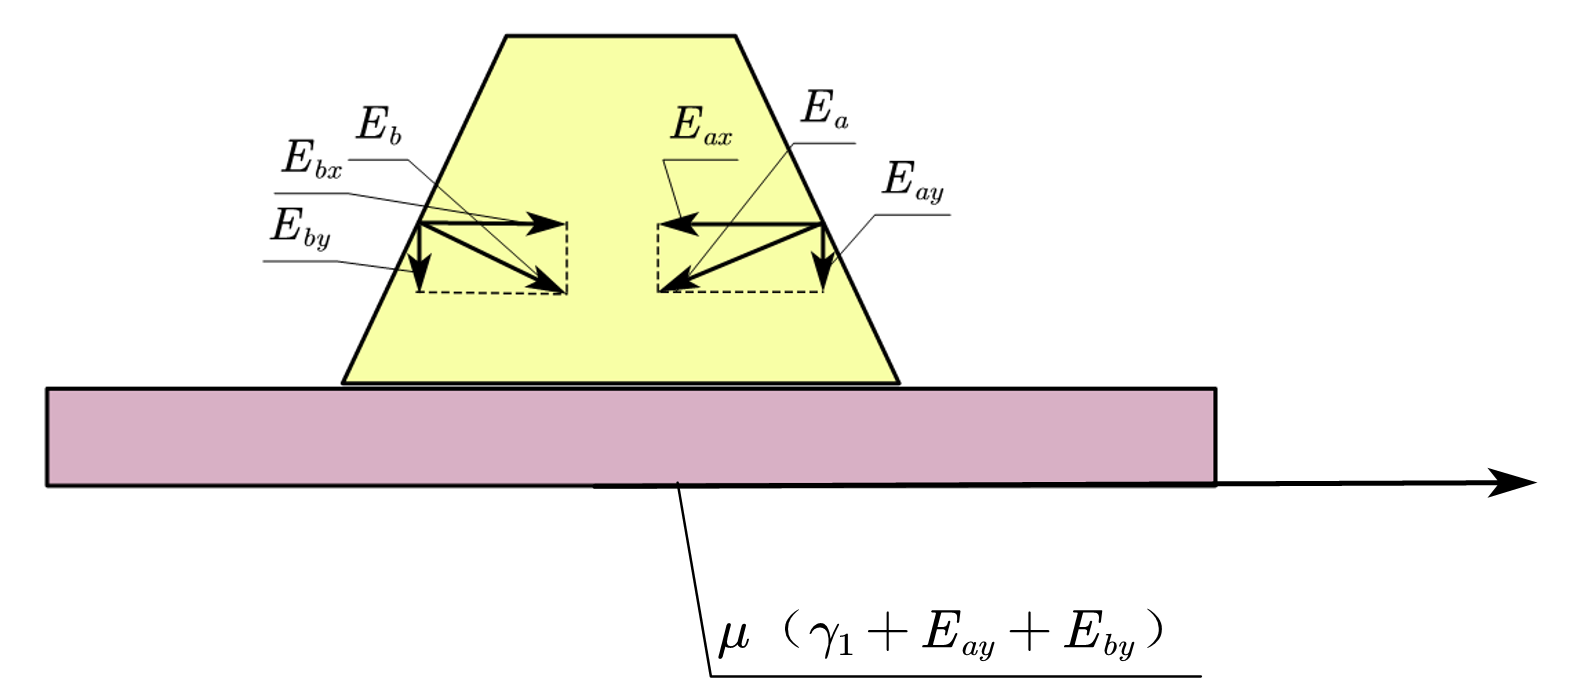
\includegraphics[width=0.5\textwidth]{受力分析1.png}
        \caption{主动土和被动土压力受力分析图}
        \label{fig:主动土和被动土压力受力分析图}
    \end{figure}

    在此基础上,我们可以得到相关力矩的分析图:
    \begin{figure}[H]
    \centering
    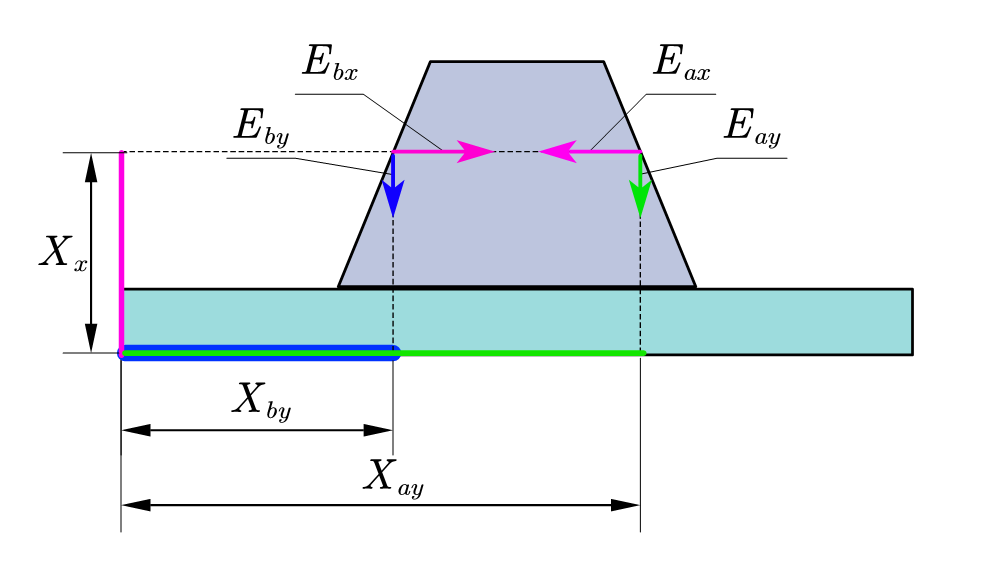
\includegraphics[width=0.5\textwidth]{力矩2.png}
    \caption{主动土和被动土压力力矩图}
    \label{fig:主动土和被动土压力力矩图}
    \end{figure}


\subsubsection{偏导求解}
为方便说明,我们定义了一个有关稳定性和抗倾覆安全系数、抗滑移安全系数的函数:

    \begin{equation}
        k_w=w_1k_s+w_2k_t
    \end{equation}
\par
其中,可以认为抗倾覆安全系数、抗滑移安全系数两者在本题中有同等重要性,即$w_1=w_2=0.5$。
则当函数分别对$\varphi$和$\alpha$求偏导时,可以分析稳定性和两个参数之间的变化规律。
我们代入在约束条件内的一组参数,即:$H$=6,$L$=2.5,$t$=0.4,$b_2$=2.5,$b_1$=0.3,$B_1$=2,$B_2$=1,$d_1$=0.3,$\beta_1$=0,$\beta$=90。得到原函数:
    \begin{equation}
        f(\alpha, \varphi) = \frac{A \cdot \cos\left(\frac{\varphi}{3}\right)}{\cos^2(\varphi)} + \frac{B}{C}
    \end{equation}

其中:
    \begin{equation*}
        A = 0.000137786596119929 \left( \sqrt{\frac{\sin(\varphi) \sin\left(\frac{4\varphi}{3}\right)}{\cos\left(\frac{\varphi}{3}\right)}} + 1 \right)^2 \cdot \left( 1655.424 + D - E \right)
    \end{equation*}

    \begin{equation*}
        B = 0.25 \left( -\frac{3628.8 \left(1 - \frac{2}{\tan(\alpha)}\right) \sin^2(\alpha-\varphi) \cos(\alpha)}{(\sqrt{F} + 1)^2 \sin^2(\alpha) \sin\left(\alpha+\frac{\varphi}{3}\right)} + 1671.408 - \frac{3142.848}{\tan(\alpha)} \right)
    \end{equation*}

    \begin{equation*}
        C = D + \frac{3628.8 \cos^2(\varphi)}{\left( \sqrt{\frac{\sin(\varphi) \sin\left(\frac{4\varphi}{3}\right)}{\cos\left(\frac{\varphi}{3}\right)}} + 1 \right)^2 \cos\left(\frac{\varphi}{3}\right)}
    \end{equation*}

    \begin{equation*}
        D = \frac{3628.8 \sin^2(\alpha-\varphi) \sin(\alpha) \sin\left(\alpha+\frac{\varphi}{3}\right)}{(\sqrt{F} + 1)^2}
    \end{equation*}

    \begin{equation*}
        E = \frac{2177.28 \sin^2(\alpha-\varphi) \cos(\alpha)}{(\sqrt{F} + 1)^2 \sin^2(\alpha) \sin\left(\alpha+\frac{\varphi}{3}\right)}
    \end{equation*}

    \begin{equation*}
        F = \frac{\sin(\varphi) \sin\left(\frac{4\varphi}{3}\right)}{\sin(\alpha) \sin\left(\alpha+\frac{\varphi}{3}\right)}
    \end{equation*}


接下来,我们对上面的原函数依次求偏导,可以得到:
    \begin{figure}[H]
    \centering
    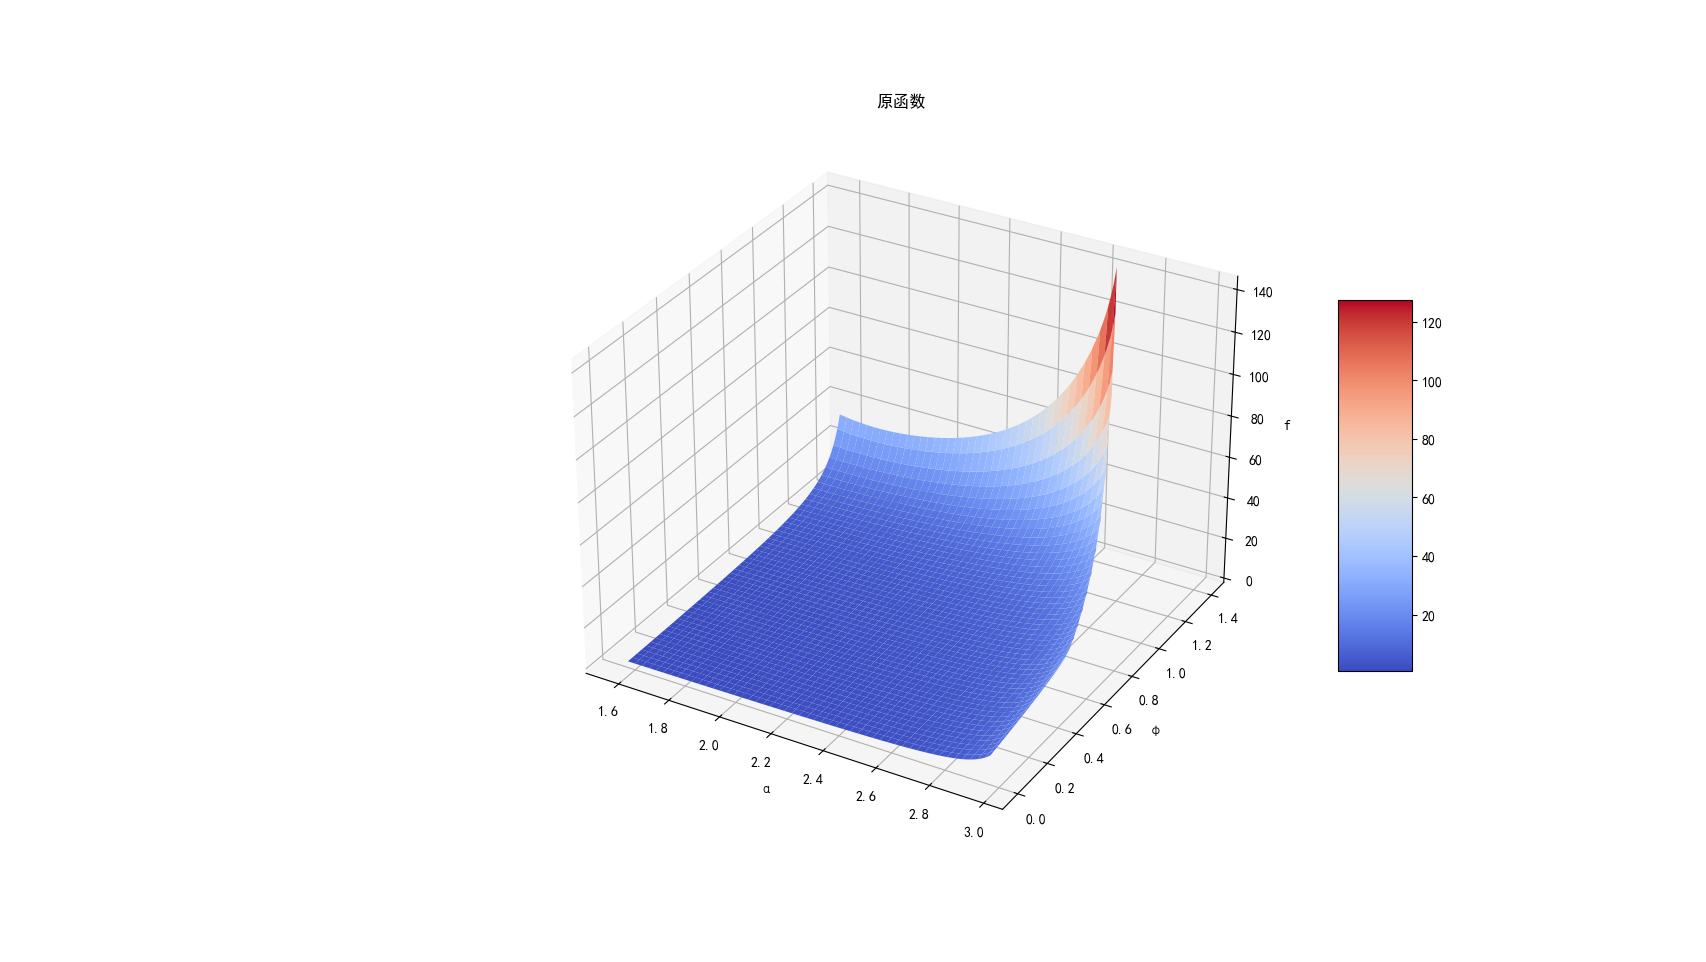
\includegraphics[width=0.8\textwidth]{原函数_1.png}
    \caption{原函数关于$\alpha$和$\varphi$关系图}
    \label{fig:原函数关于alpha和phi关系图}
    \end{figure}

    \begin{figure}[H]
    \centering
    \subcaptionbox{函数关于$\alpha$偏导\label{fig:函数关于alpha偏导}}
    {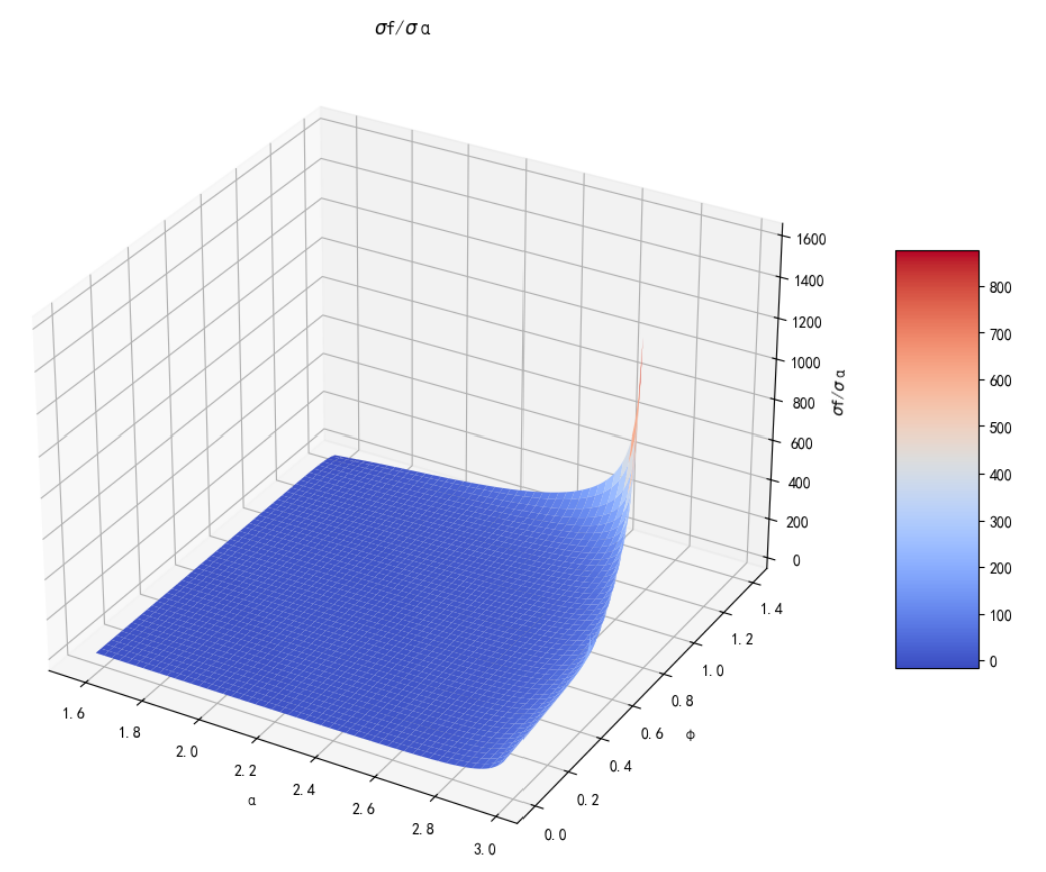
\includegraphics[width=.4\textwidth]{函数关于af偏导_1.png}}
    \subcaptionbox{函数关于$\varphi$偏导\label{fig:函数关于phi偏导}}
    {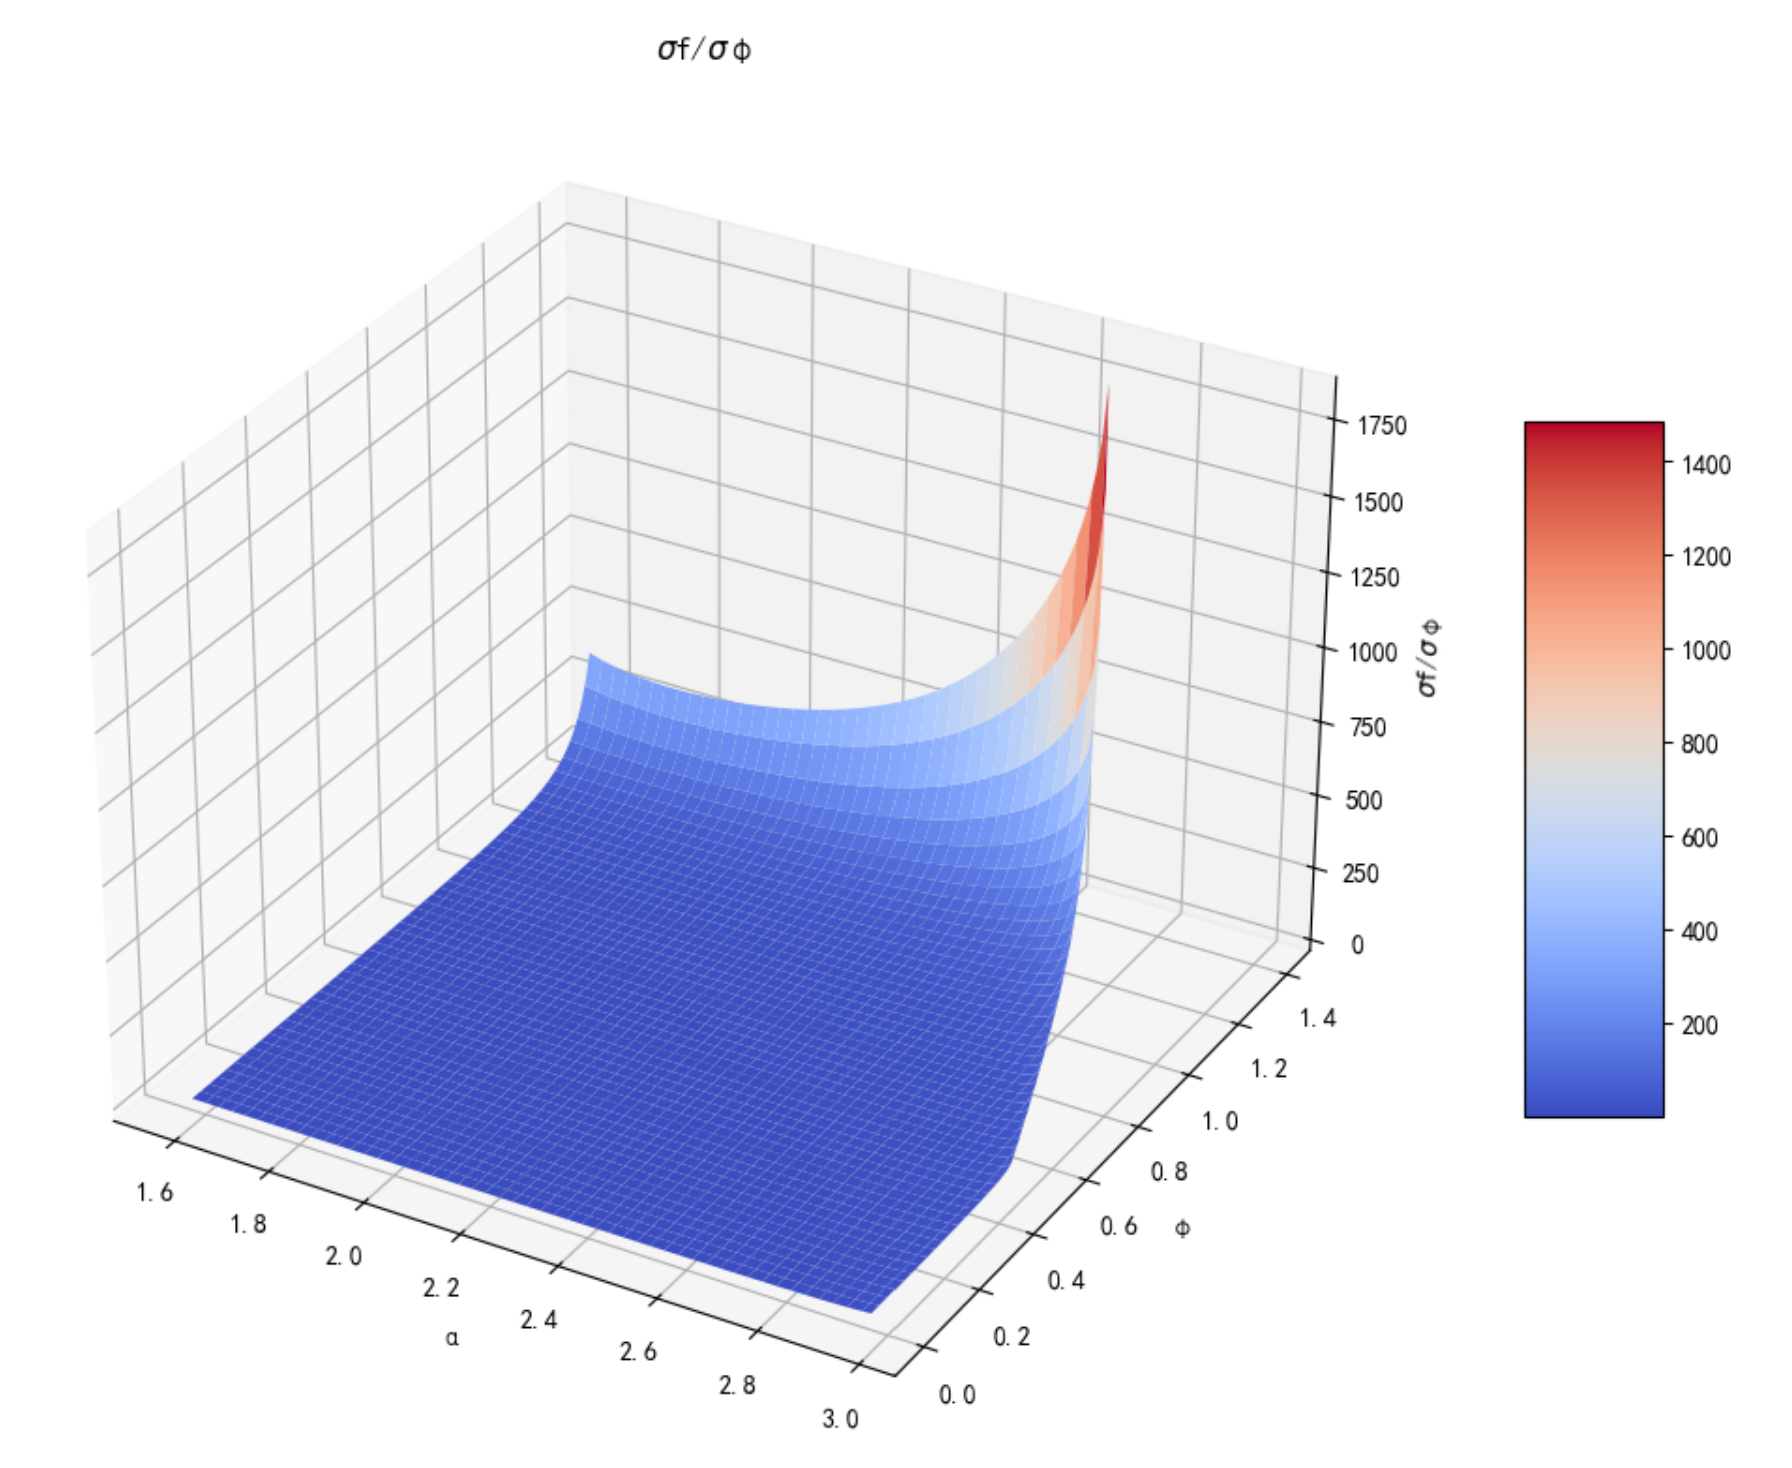
\includegraphics[width=.4\textwidth]{函数关于sita偏导_1.png}}
    \caption{函数关于$\alpha$和$\varphi$偏导}\label{fig:双图}
    \end{figure}


从图\ref{fig:原函数关于alpha和phi关系图}和图\ref{fig:双图}呈现的函数关系与偏导结果可以清晰看出,挡土墙的整体稳定性与填土内摩擦角$\varphi$、墙面板与墙趾板的夹角$\alpha$均呈现显著的正相关关系。具体而言,当填土内摩擦角$\varphi$增大时,土体颗粒间的咬合作用增强,抗剪强度提升,使得主动土压力系数$K_a$减小,墙后土体对挡土墙的侧向推力减弱,同时被动土压力系数$K_b$增大,墙前土体提供的抗倾覆与抗滑移阻力增强,最终表现为抗倾覆安全系数$K_t$和抗滑移安全系数$K_s$的同步提高,稳定性随之增强。
\par
另一方面,当墙面板与墙趾板的夹角$\alpha$增大时(即墙面板倾斜角度更平缓),墙面板与土体的接触面积增加,土压力的竖向分力$E_{a,y}$增大,不仅通过自重与摩擦力提升了抗滑移能力,还使合力作用点向墙趾方向偏移,减小了倾覆力矩的力臂,间接提高了抗倾覆安全系数。这种正相关关系在参数取值范围内呈现连续且单调的变化趋势,说明合理增大填土内摩擦角(如通过改良填土性质)或优化墙面板与墙趾板的夹角设计,均可成为提升挡土墙稳定性的有效途径。


% \begin{align*}
% \frac{\partial f}{\partial \alpha} &= \frac{3 \left( K_1 + K_2 + K_3 + K_4 + K_5 + K_6 + K_7 + K_8 \right)}{2H \cdot M} \\
% &\quad + \frac{3 \cdot N \cdot P}{2H \cdot M^2} \\
% &\quad + \frac{1.0 \cdot Q \cdot \cos^2(btp) \cos\left(btp + \frac{\varphi}{3}\right)}{H^2 y_2 (4L + 3t) \sin(bt) \cos^2(btp - \varphi)}
% \end{align*}

% \begin{align*}
% K_1 &= -\frac{3 B_1 H^2 t y_1 \left(-\tan^2(\alpha) - 1\right)}{2 \tan^2(\alpha)}, \\
% K_2 &= \frac{0.166666666666667 H^3 y_2 (4L + 3t) \left(-\tan^2(\alpha) - 1\right) \sin^2(\alpha - \varphi) \cos(\alpha)}{(\sqrt{F} + 1)^2 \sin^2(\alpha) \sin\left(\alpha + \frac{\varphi}{3}\right) \tan^2(\alpha)}, \\
% K_3 &= \frac{1.0 H^2 y_2 \sqrt{F} \left(B_2 - \frac{H}{3 \tan(\alpha)}\right) (4L + 3t) \cdot S \cdot \sin(bt_1 - \alpha) \sin^2(\alpha - \varphi) \cos(\alpha)}{(\sqrt{F} + 1)^3 \sin^2(\alpha) \sin\left(\frac{4\varphi}{3}\right) \sin(bt_1 - \varphi)}, \\
% K_4 &= \frac{0.5 H^2 y_2 \left(B_2 - \frac{H}{3 \tan(\alpha)}\right) (4L + 3t) \sin^2(\alpha - \varphi)}{(\sqrt{F} + 1)^2 \sin(\alpha) \sin\left(\alpha + \frac{\varphi}{3}\right)}, \\
% K_5 &= \frac{0.5 H^2 y_2 \left(B_2 - \frac{H}{3 \tan(\alpha)}\right) (4L + 3t) \sin^2(\alpha - \varphi) \cos(\alpha) \cos\left(\alpha + \frac{\varphi}{3}\right)}{(\sqrt{F} + 1)^2 \sin^2(\alpha) \sin^2\left(\alpha + \frac{\varphi}{3}\right)}, \\
% K_6 &= -\frac{1.0 H^2 y_2 \left(B_2 - \frac{H}{3 \tan(\alpha)}\right) (4L + 3t) \sin(\alpha - \varphi) \cos(\alpha) \cos(\alpha - \varphi)}{(\sqrt{F} + 1)^2 \sin^2(\alpha) \sin\left(\alpha + \frac{\varphi}{3}\right)}, \\
% K_7 &= \frac{1.0 H^2 y_2 \left(B_2 - \frac{H}{3 \tan(\alpha)}\right) (4L + 3t) \sin^2(\alpha - \varphi) \cos^2(\alpha)}{(\sqrt{F} + 1)^2 \sin^3(\alpha) \sin\left(\alpha + \frac{\varphi}{3}\right)}, \\
% K_8 &= \frac{H (4L + 3t) (b_1 + b_2) \left(- \frac{H (2b_1 + b_2) \left(-\tan^2(\alpha) - 1\right)}{\tan^2(\alpha)} - \frac{H (b_1 + 2b_2) \left(-\tan^2(\alpha) - 1\right)}{3(b_1 + b_2) \tan^2(\alpha)}\right)}{2}, \\
% M &= \frac{0.5 H^2 y_2 (4L + 3t) \sin(bt) \cos^2(btp - \varphi)}{\left(\sqrt{- \frac{\sin\left(\frac{4\varphi}{3}\right) \sin(bt_1 - \varphi)}{\cos(bt_1 - btp) \cos\left(btp + \frac{\varphi}{3}\right)}} + 1\right)^2 \cos^2(btp) \cos\left(btp + \frac{\varphi}{3}\right)} + \frac{0.5 H^2 y_2 (4L + 3t) \sin^2(\alpha - \varphi)}{(\sqrt{F} + 1)^2 \sin(\alpha) \sin\left(\alpha + \frac{\varphi}{3}\right)}, \\
% N &= \frac{1.0 H^2 y_2 \sqrt{F} (4L + 3t) \cdot S \cdot \sin(bt_1 - \alpha) \sin^2(\alpha - \varphi)}{(\sqrt{F} + 1)^3 \sin(\alpha) \sin\left(\frac{4\varphi}{3}\right) \sin(bt_1 - \varphi)} + \frac{0.5 H^2 y_2 (4L + 3t) \sin^2(\alpha - \varphi) \cos\left(\alpha + \frac{\varphi}{3}\right)}{(\sqrt{F} + 1)^2 \sin(\alpha) \sin^2\left(\alpha + \frac{\varphi}{3}\right)} - \frac{1.0 H^2 y_2 (4L + 3t) \sin(\alpha - \varphi) \cos(\alpha - \varphi)}{(\sqrt{F} + 1)^2 \sin(\alpha) \sin\left(\alpha + \frac{\varphi}{3}\right)} + \frac{0.5 H^2 y_2 (4L + 3t) \sin^2(\alpha - \varphi) \cos(\alpha)}{(\sqrt{F} + 1)^2 \sin^2(\alpha) \sin\left(\alpha + \frac{\varphi}{3}\right)}, \\
% P &= \frac{3 B_1 H t y_1 \left(\frac{B_1}{3} + B_2 - \frac{H}{\tan(\alpha)} - \frac{2H}{3 \tan(bt)} + b_1\right)}{2} - \frac{0.5 H^2 y_2 \left(B_2 - \frac{H}{3 \tan(\alpha)}\right) (4L + 3t) \sin^2(\alpha - \varphi) \cos(\alpha)}{(\sqrt{F} + 1)^2 \sin^2(\alpha) \sin\left(\alpha + \frac{\varphi}{3}\right)} - \frac{0.5 H^2 y_2 (4L + 3t) \left(B_2 + \frac{H}{3 \tan(bt)} + b_2\right) \cos(bt) \cos^2(btp - \varphi)}{\left(\sqrt{- \frac{\sin\left(\frac{4\varphi}{3}\right) \sin(bt_1 - \varphi)}{\cos(bt_1 - btp) \cos\left(btp + \frac{\varphi}{3}\right)}} + 1\right)^2 \cos^2(btp) \cos\left(btp + \frac{\varphi}{3}\right)} + \frac{H (4L + 3t) (b_1 + b_2) \left(B_2 - \frac{H (2b_1 + b_2)}{\tan(\alpha)} + \frac{(b_1 + 2b_2) \left(- \frac{H}{\tan(\alpha)} + b_1\right)}{3(b_1 + b_2)}\right)}{2} + \frac{d_1 y_1 (4L + 3t) (B_1 + B_2 + b_2)^2}{2}, \\
% Q &= \left(\sqrt{- \frac{\sin\left(\frac{4\varphi}{3}\right) \sin(bt_1 - \varphi)}{\cos(bt_1 - btp) \cos\left(btp + \frac{\varphi}{3}\right)}} + 1\right)^2 \left( - \frac{1.0 H^2 y_2 \sqrt{F} (4L + 3t) \cdot S \cdot \sin(bt_1 - \alpha) \sin^2(\alpha - \varphi)}{(\sqrt{F} + 1)^3 \sin(\alpha) \sin\left(\frac{4\varphi}{3}\right) \sin(bt_1 - \varphi)} - \frac{0.5 H^2 y_2 (4L + 3t) \sin^2(\alpha - \varphi) \cos\left(\alpha + \frac{\varphi}{3}\right)}{(\sqrt{F} + 1)^2 \sin(\alpha) \sin^2\left(\alpha + \frac{\varphi}{3}\right)} + \frac{1.0 H^2 y_2 (4L + 3t) \sin(\alpha - \varphi) \cos(\alpha - \varphi)}{(\sqrt{F} + 1)^2 \sin(\alpha) \sin\left(\alpha + \frac{\varphi}{3}\right)} - \frac{0.5 H^2 y_2 (4L + 3t) \sin^2(\alpha - \varphi) \cos(\alpha)}{(\sqrt{F} + 1)^2 \sin^2(\alpha) \sin\left(\alpha + \frac{\varphi}{3}\right)} + u \cdot T \right), \\
% S &= - \frac{\sin\left(\frac{4\varphi}{3}\right) \sin(bt_1 - \varphi) \cos\left(\alpha + \frac{\varphi}{3}\right)}{2 \sin(bt_1 - \alpha) \sin^2\left(\alpha + \frac{\varphi}{3}\right)} + \frac{\sin\left(\frac{4\varphi}{3}\right) \sin(bt_1 - \varphi) \cos(bt_1 - \alpha)}{2 \sin^2(bt_1 - \alpha) \sin\left(\alpha + \frac{\varphi}{3}\right)}, \\
% T &= \frac{1.0 H^2 y_2 \sqrt{F} (4L + 3t) \cdot S \cdot \sin(bt_1 - \alpha) \sin^2(\alpha - \varphi) \cos(\alpha)}{(\sqrt{F} + 1)^3 \sin^2(\alpha) \sin\left(\frac{4\varphi}{3}\right) \sin(bt_1 - \varphi)} + \frac{0.5 H^2 y_2 (4L + 3t) \sin^2(\alpha - \varphi)}{(\sqrt{F} + 1)^2 \sin(\alpha) \sin\left(\alpha + \frac{\varphi}{3}\right)} + \frac{0.5 H^2 y_2 (4L + 3t) \sin^2(\alpha - \varphi) \cos(\alpha) \cos\left(\alpha + \frac{\varphi}{3}\right)}{(\sqrt{F} + 1)^2 \sin^2(\alpha) \sin^2\left(\alpha + \frac{\varphi}{3}\right)} - \frac{1.0 H^2 y_2 (4L + 3t) \sin(\alpha - \varphi) \cos(\alpha) \cos(\alpha - \varphi)}{(\sqrt{F} + 1)^2 \sin^2(\alpha) \sin\left(\alpha + \frac{\varphi}{3}\right)} + \frac{1.0 H^2 y_2 (4L + 3t) \sin^2(\alpha - \varphi) \cos^2(\alpha)}{(\sqrt{F} + 1)^2 \sin^3(\alpha) \sin\left(\alpha + \frac{\varphi}{3}\right)}, \\
% F &= \frac{\sin\left(\frac{4\varphi}{3}\right) \sin(bt_1 - \varphi)}{\sin(bt_1 - \alpha) \sin\left(\alpha + \frac{\varphi}{3}\right)}.
% \end{align*}




%%%%%%%%%%%%%%%%%%%%%%%%%%%%%%%%%%%%%%%%%%%%%%%%%%%%%%%%%%%%% 

\section{问题二的模型的建立和求解}
\subsection{参数改变}
\subsubsection{几何参数的新增}
我们在问题一的基础上,新规定了以下重要的几何参数:$L$表示底桩的半径,约束条件为大于0.3米;
$D$表示深度,约束条件为$\frac{H}{5}$到$\frac{H}{2}$;
$L_2$表示间隔,其约束条件为$\frac{L_1}{5}$到$\frac{2L_1}{3}$。
示例图如下:

\begin{figure}[H]
\centering
\subcaptionbox{底桩主视图\label{fig:底桩主视图}}
{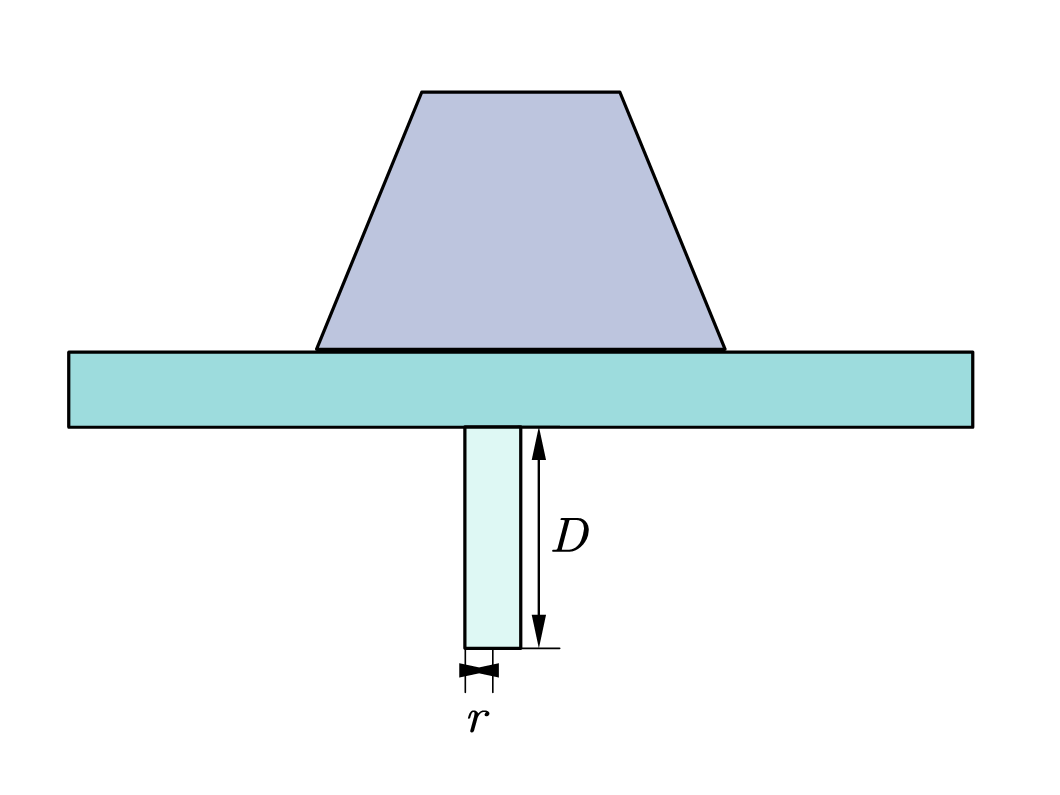
\includegraphics[width=.4\textwidth]{底桩1.png}}
\subcaptionbox{底桩侧视图\label{fig:底桩侧视图}}
{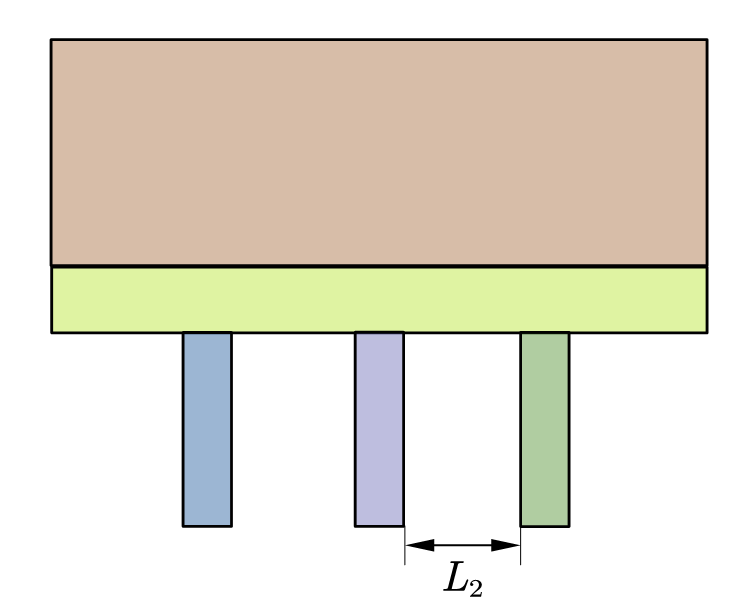
\includegraphics[width=.4\textwidth]{底桩2.png}}
\caption{底桩主视图及侧视图}\label{fig:底桩主视图及侧视图}
\end{figure} 

\subsubsection{荷载参数的新增}
同样,我们在问题一的基础上,新规定了以下重要的荷载参数:
$F_p$表示底柱对土层的侧向摩擦力,$T_f$表示单位摩擦力,则有
    \begin{equation}
        F_{px}=\int_{0}^{\frac{\pi }{2} }\pi rLT_fcos\theta  \mathrm{d}\theta=\pi rLT_f
    \end{equation}
同时,我们更新了有底桩侧向摩擦力的受力分析图:

    \begin{figure}[H]
        \centering
        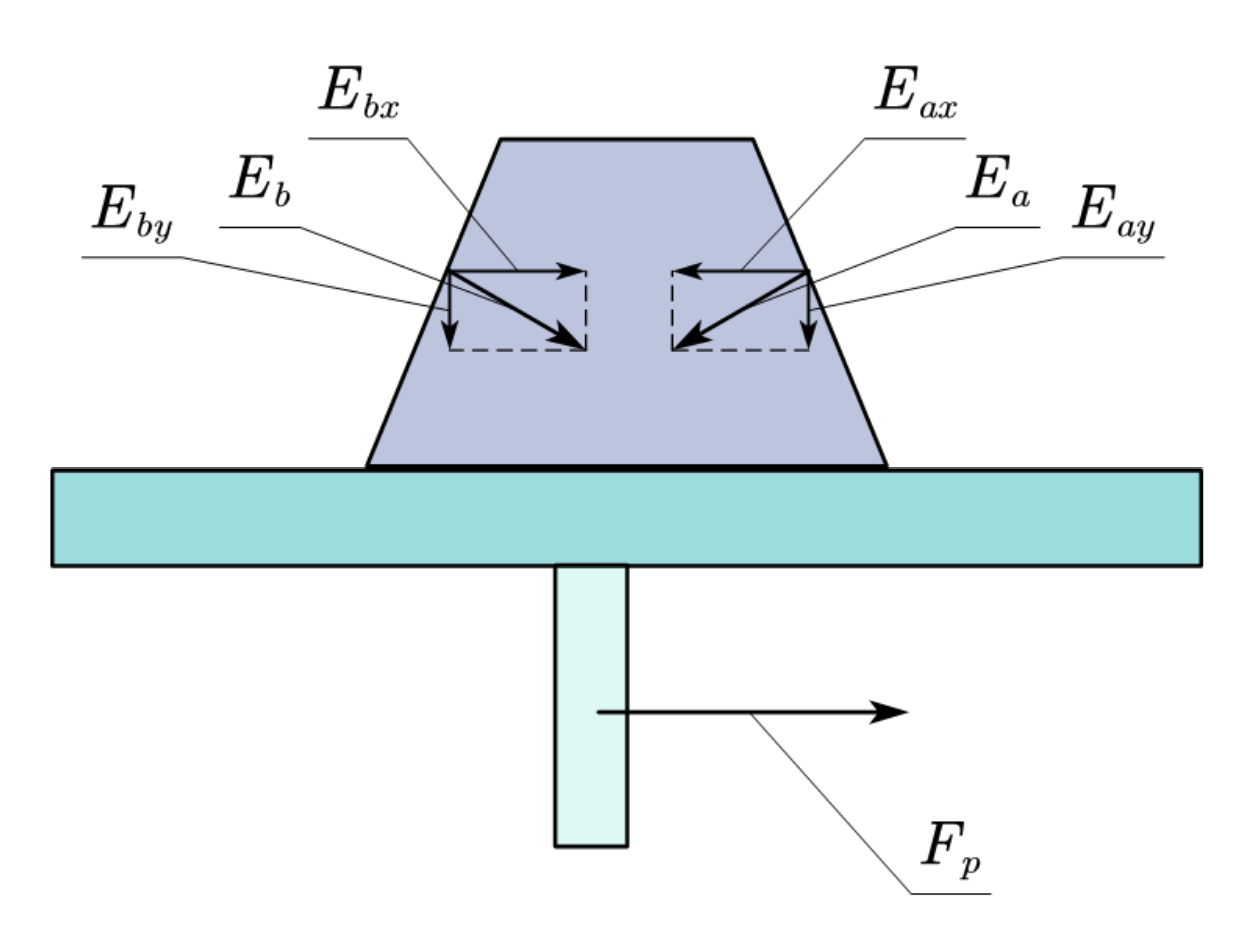
\includegraphics[width=0.5\textwidth]{受力分析2.png}
        \caption{有底桩侧向摩擦力的受力分析图}
        \label{fig:有底桩侧向摩擦力的受力分析图}
    \end{figure}

在受力分析的基础上,我们可以得到相关力矩的分析图:
    \begin{figure}[H]
    \centering
    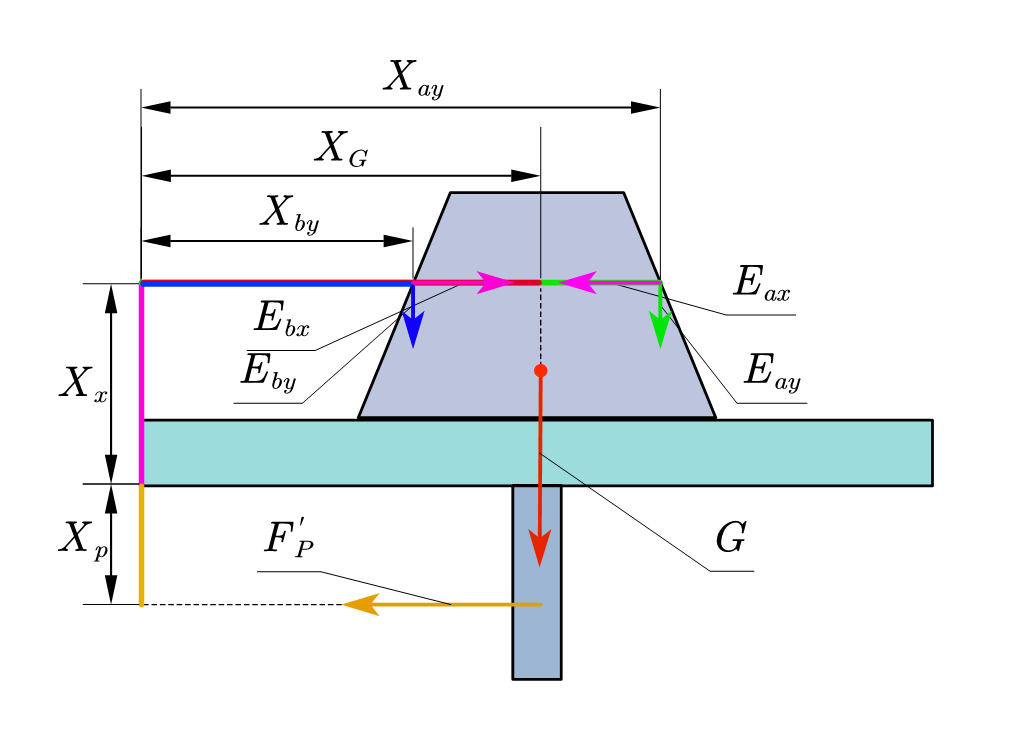
\includegraphics[width=0.5\textwidth]{受力分析3.png}
    \caption{有底桩侧向摩擦力的力矩分析图}
    \label{fig:有底桩侧向摩擦力的力矩分析图}
    \end{figure}
\subsection{规律的变化}
在模型一的基础上,我们发现增加底桩后,$K_s$和$K_t$发生了以下变化:

    \begin{equation}
        \left\{
            \begin{aligned}
                &K_s^{\prime}=\frac{[\gamma_1 V+(4L+3t)E_{ay}+(4L+3t)E_{by}]\mu +n\pi rLT_f+(4l+3t)E_{bx}}{(4L+3t)E_{ax}} \\
                &K_t^{\prime} = \frac{{G_{ax}}X_G+n\gamma_1\pi rLT_f(B_L+\frac{b_2}{2}) + (4l + 3t)(E_{ay}X_{ay} + E_{by}X_{by})n\pi rLT_f+\frac{b_2}{2}}{(4L+3t)(E_{ax}-E_{bx})\frac{H}{3}}
            \end{aligned}
        \right.
    \end{equation}
    \par
上述式子中,相对于第一问的模型,我们主要重新更新了挡土墙的体积公式,并且添加了有关底柱的相关参数。
代入式子中,我们可以得到以下原函数公式:
    \begin{equation}
        f(\alpha, \beta) = \frac{3 \cdot A}{2H \cdot B} + \frac{C \cdot D}{H^2 y_2 (4L + 3t) \sin^2(\beta - \varphi)}
    \end{equation}\par
其中:

\begin{equation*}
    A = 0.000137786596119929 \left( \sqrt{\frac{\sin(\varphi) \sin\left(\frac{4\varphi}{3}\right)}{\cos\left(\frac{\varphi}{3}\right)}} + 1 \right)^2 \cdot \left( 1655.424 + D - E \right)
\end{equation*}

\begin{equation*}
    B = 0.25 \left( -\frac{3628.8 \left(1 - \frac{2}{\tan(\alpha)}\right) \sin^2(\alpha-\varphi) \cos(\alpha)}{(\sqrt{F} + 1)^2 \sin^2(\alpha) \sin\left(\alpha+\frac{\varphi}{3}\right)} + 1671.408 - \frac{3142.848}{\tan(\alpha)} \right)
\end{equation*}

\begin{equation*}
    C = D + \frac{3628.8 \cos^2(\varphi)}{\left( \sqrt{\frac{\sin(\varphi) \sin\left(\frac{4\varphi}{3}\right)}{\cos\left(\frac{\varphi}{3}\right)}} + 1 \right)^2 \cos\left(\frac{\varphi}{3}\right)}
\end{equation*}

\begin{equation*}
    D = \frac{3628.8 \sin^2(\alpha-\varphi) \sin(\alpha) \sin\left(\alpha+\frac{\varphi}{3}\right)}{(\sqrt{F} + 1)^2}
\end{equation*}

\begin{equation*}
    E = \frac{2177.28 \sin^2(\alpha-\varphi) \cos(\alpha)}{(\sqrt{F} + 1)^2 \sin^2(\alpha) \sin\left(\alpha+\frac{\varphi}{3}\right)}
\end{equation*}

\begin{equation*}
    F = \frac{\sin(\varphi) \sin\left(\frac{4\varphi}{3}\right)}{\sin(\alpha) \sin\left(\alpha+\frac{\varphi}{3}\right)}
\end{equation*}

在函数分别对$\alpha$ 和$\beta$ 求偏导后,我们可以得到:
    \begin{figure}[H]
        \centering
        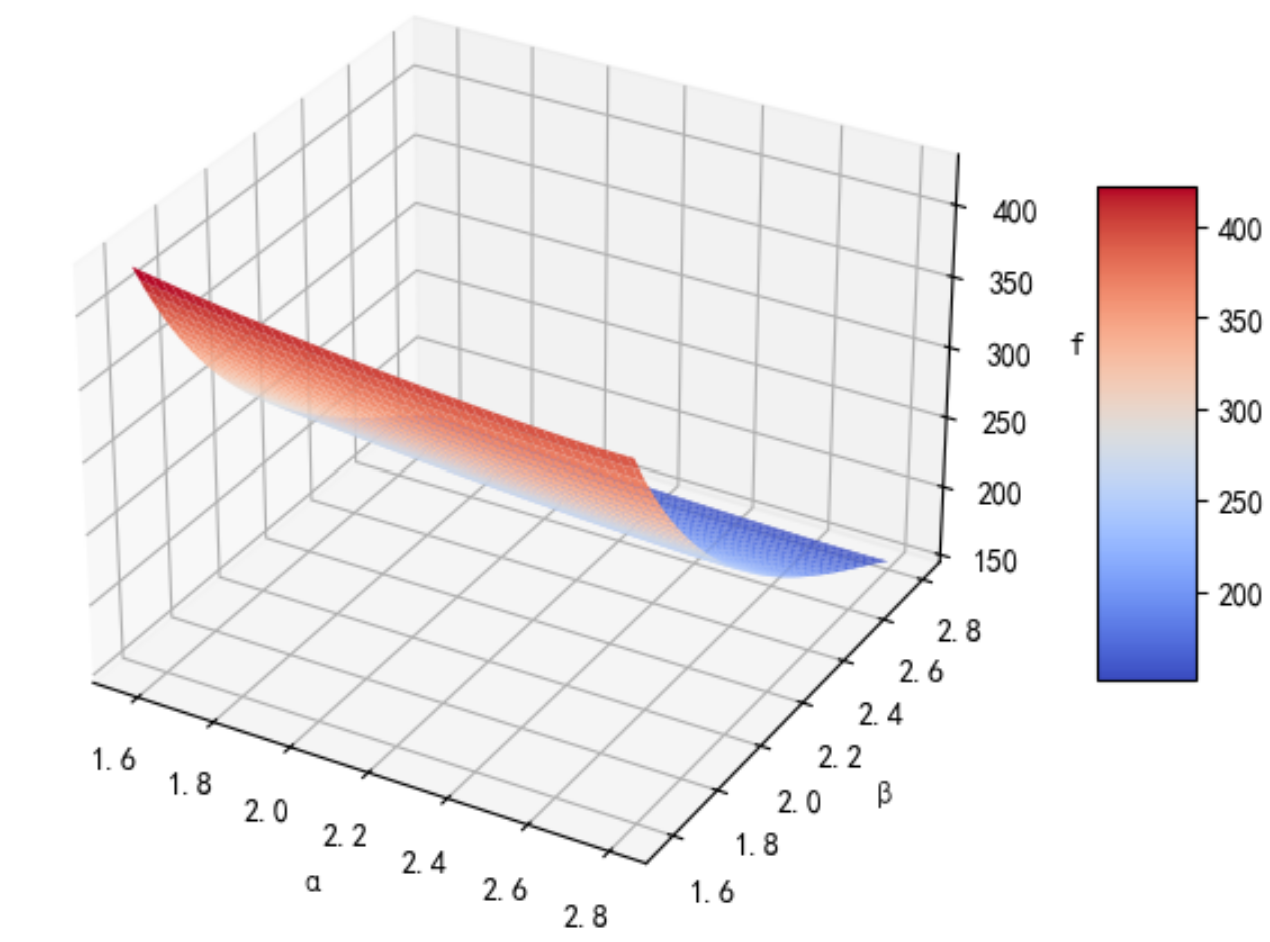
\includegraphics[width=0.5\textwidth]{原函数_2.png}
        \caption{原函数关于$\alpha$和$\beta$关系图}
        \label{fig:原函数关于alpha和phi关系图}
    \end{figure}

    \begin{figure}[H]
        \centering
        \subcaptionbox{函数关于$\alpha$偏导\label{fig:函数关于alpha偏导2}}
        {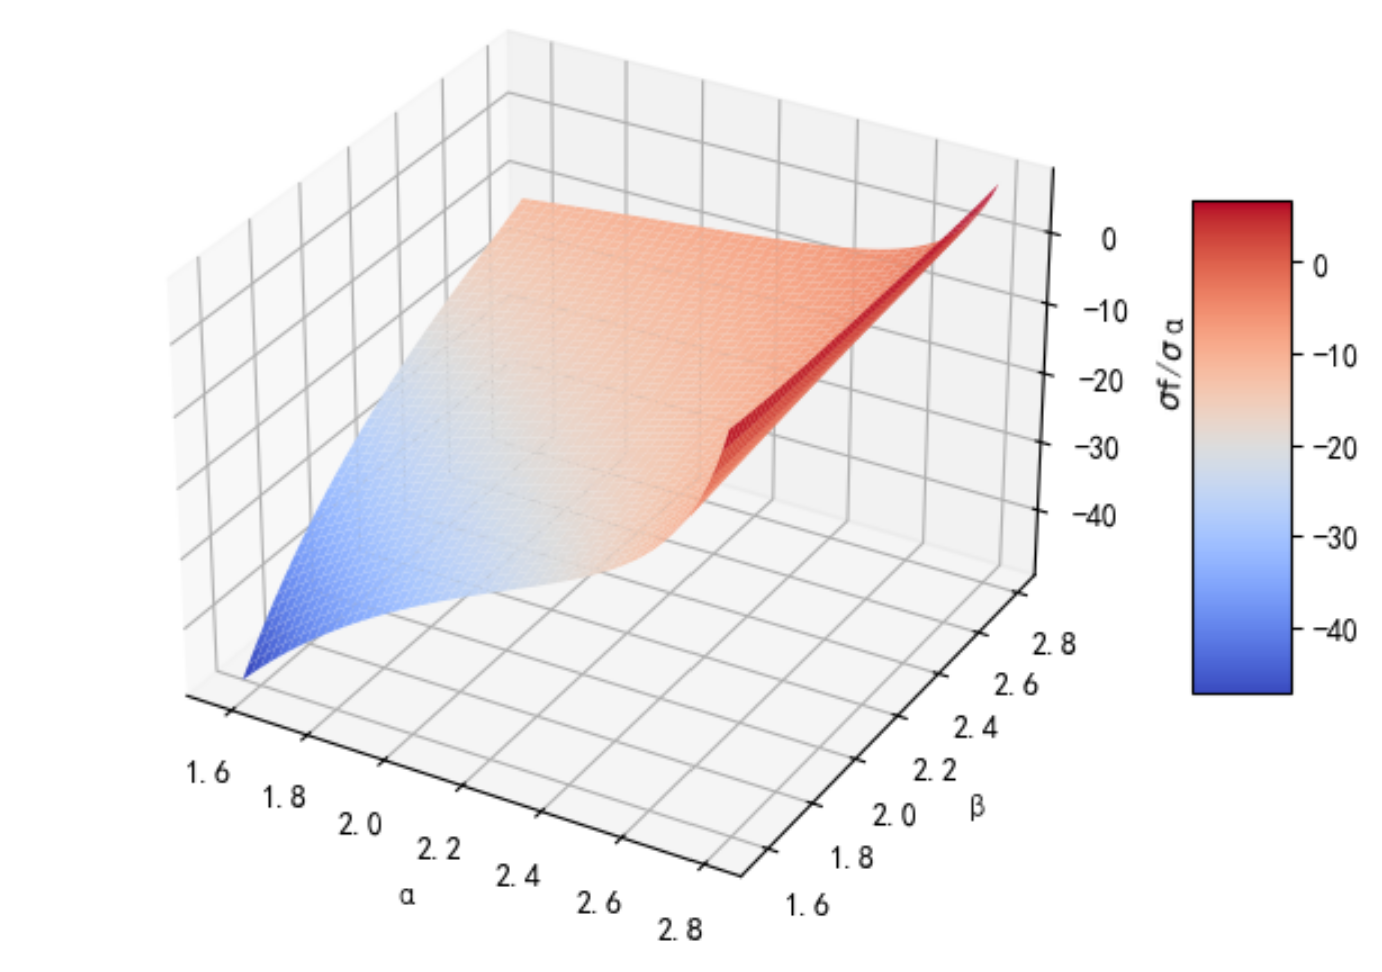
\includegraphics[width=.4\textwidth]{函数关于af偏导_2.png}}
        \subcaptionbox{函数关于$\beta$偏导\label{fig:函数关于beta偏导2}}
        {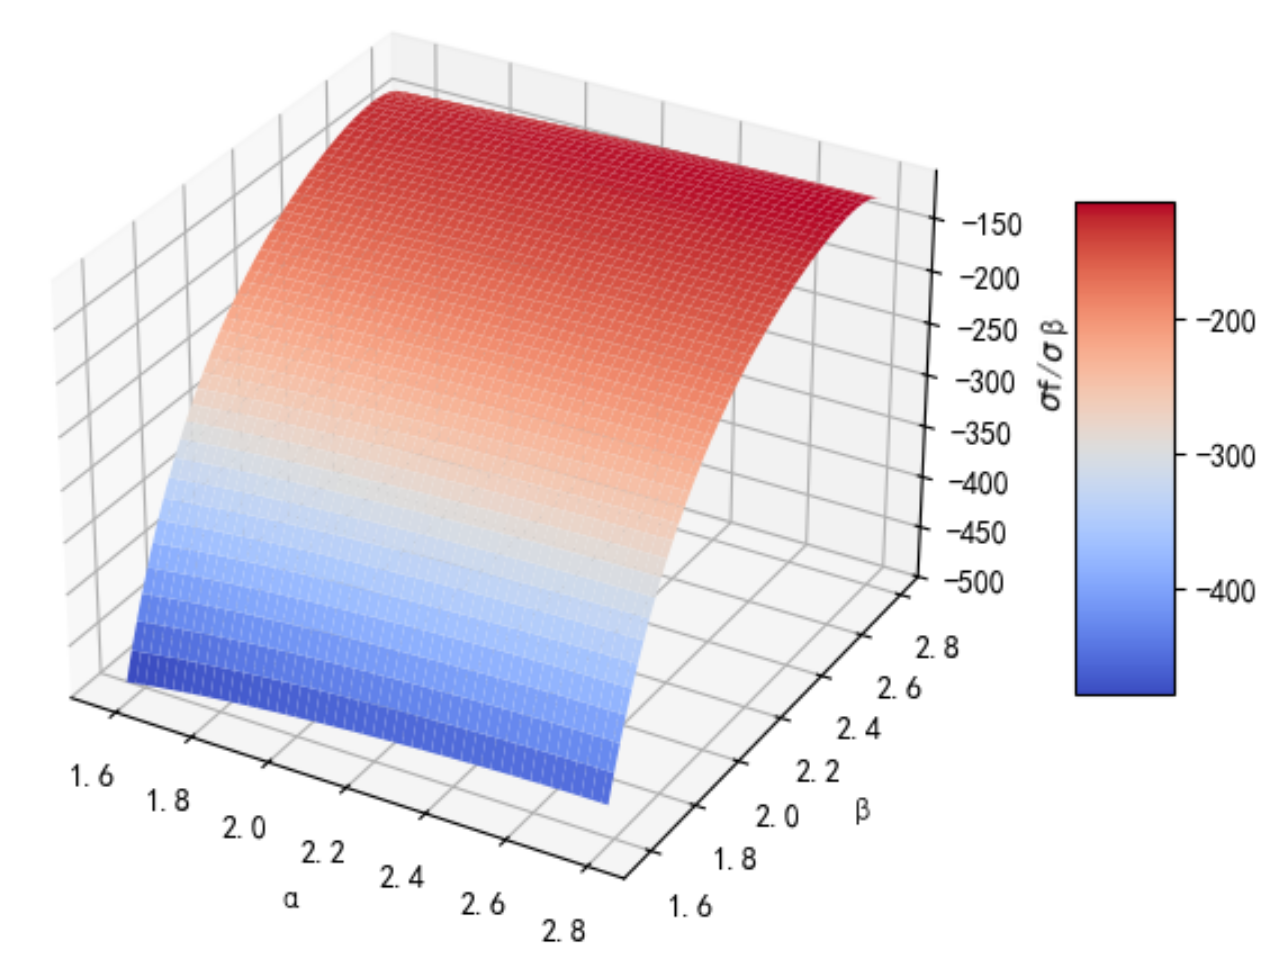
\includegraphics[width=.4\textwidth]{函数关于beta偏导_2.png}}
        \caption{函数关于$\alpha$和$\beta$偏导}\label{fig:双图}
    \end{figure}

从图\ref{fig:原函数关于alpha和phi关系图}中可以清晰观察到挡土墙稳定性与几何参数之间的关系呈现出显著的规律性。稳定性指标(由函数$f$表示)随$\alpha$(墙面板与墙趾板的夹角)的增大而单调递增,当$\alpha$从1.6增加到2.8时,稳定性指标从约200增加到400,增幅达100\%。偏导数$\frac{\partial f}{\partial \alpha}$始终为负值,表明$\alpha$每增加一个单位,稳定性指标将减少约40个单位。这一趋势与挡土墙工程中"增大墙背倾角可提高稳定性"的经验规律相符。

与此同时,稳定性指标随$\beta$(墙面板与墙踵板的夹角)的增大而单调递减,当$\beta$从1.6增加到2.8时,稳定性指标从约400减少到200,降幅达50\%。偏导数$\frac{\partial f}{\partial \beta}$始终为负值,且绝对值大于$\frac{\partial f}{\partial \alpha}$,表明$\beta$对稳定性的影响比$\alpha$更显著。如图\ref{fig:双图}所示,在$\alpha \approx 2.8$,$\beta \approx 1.6$附近,稳定性指标达到最大值约400;而在$\alpha \approx 1.6$,$\beta \approx 2.8$附近,稳定性指标降至最小值约200。两个参数对稳定性的影响呈现相反趋势,这为挡土墙的优化设计提供了重要依据。
\subsection{基于非线性规划的钢筋位置稳定性最优化设计模型}

\subsubsection{目标函数的建立}
同问题一,我们在建立模型时,主要考虑抗倾覆安全系数和抗滑移安全系数对总体稳定性影响。
因此,在上述模型上,我们针对钢筋相关参数做了进一步扩充,可以得到:

    \begin{equation}
        \begin{aligned}
            \begin{cases}
                k_s'' &= \dfrac{[\gamma_1 V + (4L + 3t)E_{ay} + (4L + 3t)E_{by}]\mu + n\pi r L T_f + (4l + 3t)E_{bx}}{(4L + 3t)E_{ax}} \\
                k_t'' &= \dfrac{G_{ax}' X_G' + n\gamma_1 \pi r L T_f \left(B_L + \dfrac{b_2}{2}\right) + (4l + 3t)\left(E_{ay}X_{ay} + E_{by}X_{by}\right)}{(4L + 3t)\left(E_{ax} - E_{bx}\right)\dfrac{H}{3}} \\
                & \quad + \dfrac{n\pi r \dfrac{D^2}{2}T_f + \dfrac{b_2}{2} + 2T_h(y + d_1)}{(4L + 3t)\left(E_{ax} - E_{bx}\right)\dfrac{H}{3}}
            \end{cases}
            \end{aligned}
        \label{eq:stability}
    \end{equation}

将新的参数代入公式16中,可以得到目标函数:
    \begin{equation}
        k_w''=w_1k_s''+w_2k_t''
    \end{equation}
    \par
其中,可以认为抗倾覆安全系数、抗滑移安全系数两者在本模型中同等重要,即$w_1=w_2=0.5$。

\subsubsection{钢筋约束条件的建立}
我们在建立模型时,考虑到本模型相较以上模型最大进步是在新增了钢筋这一约束条件,因此在考虑约束时重点考虑钢筋的影响。
我们约定了$T_h$为钢筋水平拉力,则对应的拉力应该比钢筋内部摩擦力和挡土墙外部摩擦力最小值要小。
则有:

\begin{equation}
    T_h\le min(\pi d_a\tau _t,F_p+f_\text{地} )
\end{equation}
\par
其中:
$$f_\text{地}=[\gamma _1V+\gamma _2V_j+(E_{a,y}+ E_{b,y})(4L+3t)]\mu ,\quad F_P=\pi rL_a\tau f$$


同时,我们认为钢筋应该在挡土墙内部,因此为方便后续模型求解,我们建立如下坐标系:

    \begin{figure}[H]
    \centering
    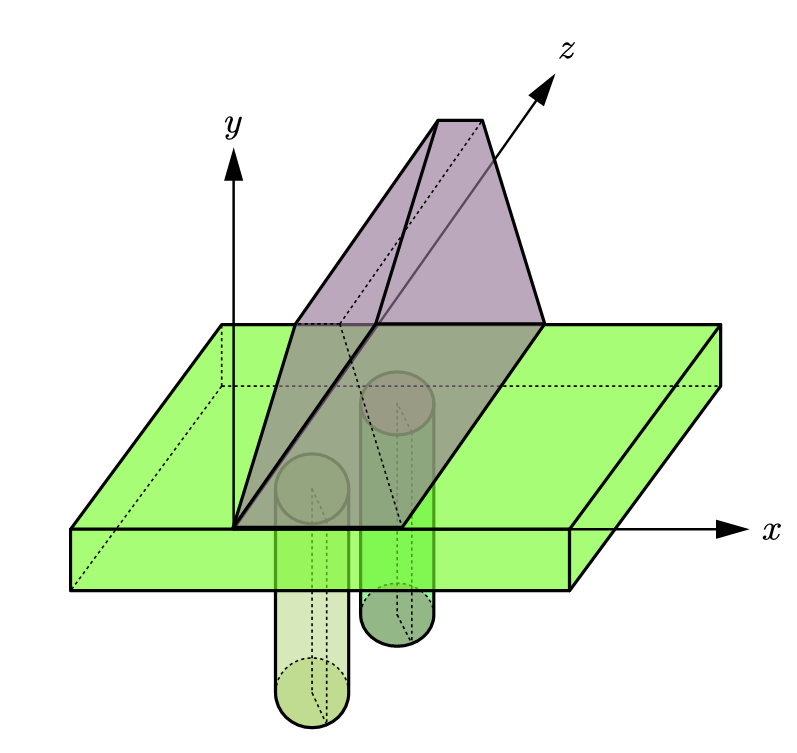
\includegraphics[width=0.5\textwidth]{坐标系2.png}
    \caption{坐标系参考图}
    \label{fig:{坐标系参考图}}
    \end{figure}

其中,我们以挡土墙主视图中梯形左下为坐标原点,水平向右为x轴,竖直向上为y轴,同时贯深向内部为z轴,建立直角坐标系。
因此,有以下约束:
    \begin{equation}
            \left\{\begin{matrix} 
                \frac{|tanx+y|}{\sqrt{tan\alpha^2+1} } \ge 0.04\\
                \frac{|-tan\beta \cdot x-y+tan\beta(b-\frac{H}{tan\beta}- \frac{H}{tan\alpha})|}{\sqrt{tan\beta^2+1} }\ge 0.04 
            \end{matrix}\right.  
    \end{equation}
    \par
其中,$x$表示钢筋的横坐标,$y$表示钢筋的纵坐标。
并且我们为了让钢筋在挡土墙中,对不同分段$(x,y)$进行了分段约束:
    \begin{equation}
        \left\{\begin{matrix} 
            x\in [0,-\frac{H}{tan\alpha } ],y\in [0.04, -tan\alpha ] \\
            x\in [-\frac{H}{tan\alpha } ,b_1-\frac{H}{tan\alpha } ],y\in [0.04, H-0.04 ] \\
            x\in [b_1-\frac{H}{tan\alpha } ,b_1-\frac{H}{tan\alpha }- \frac{H}{tan\beta }],y\in [0.04, -tan\beta \cdot x+tan\beta(b-\frac{H}{tan\beta}- \frac{H}{tan\alpha} ] \\
        \end{matrix}\right.  
    \end{equation}

上述式子中,我们对钢筋的横纵坐标进行了约束,但是实际上钢筋的横贯位置也是需要考虑的。因此我们查阅有关混凝土结构设计方案\upcite{中华人民共和国建设部2002GB},得到以下约束:
    \begin{equation}
        \alpha \cdot \frac{f_y}{f_t} \cdot d\le L_a\le \frac{4L+3t}{2} 
    \end{equation}\par
式中:
    \begin{itemize}
        \item $L_{a,\text{min}}$--最小锚固长度(m),为保证拉筋在土体中不发生拔出破坏所需的最小埋置深度;
        \item $\alpha$--锚固长度修正系数,无量纲,其取值与拉筋类型及锚固条件密切相关。我们取得的带肋钢筋,$\alpha$通常取0.14;
        \item $f_y$--拉筋屈服强度(MPa),取决于钢筋的材质和等级。我们使用的HRB400级钢筋的屈服强度标准值为400MPa;
        \item $f_t$--墙体混凝土轴心抗拉强度设计值(MPa),与混凝土强度等级相关。对于C30混凝土,$f_t$取1.43MPa;
        \item $d$--拉筋直径(m),为拉筋的公称外径。
    \end{itemize}

下图所示为我们加入拉筋后的示意图:
    \begin{figure}[H]
        \centering
        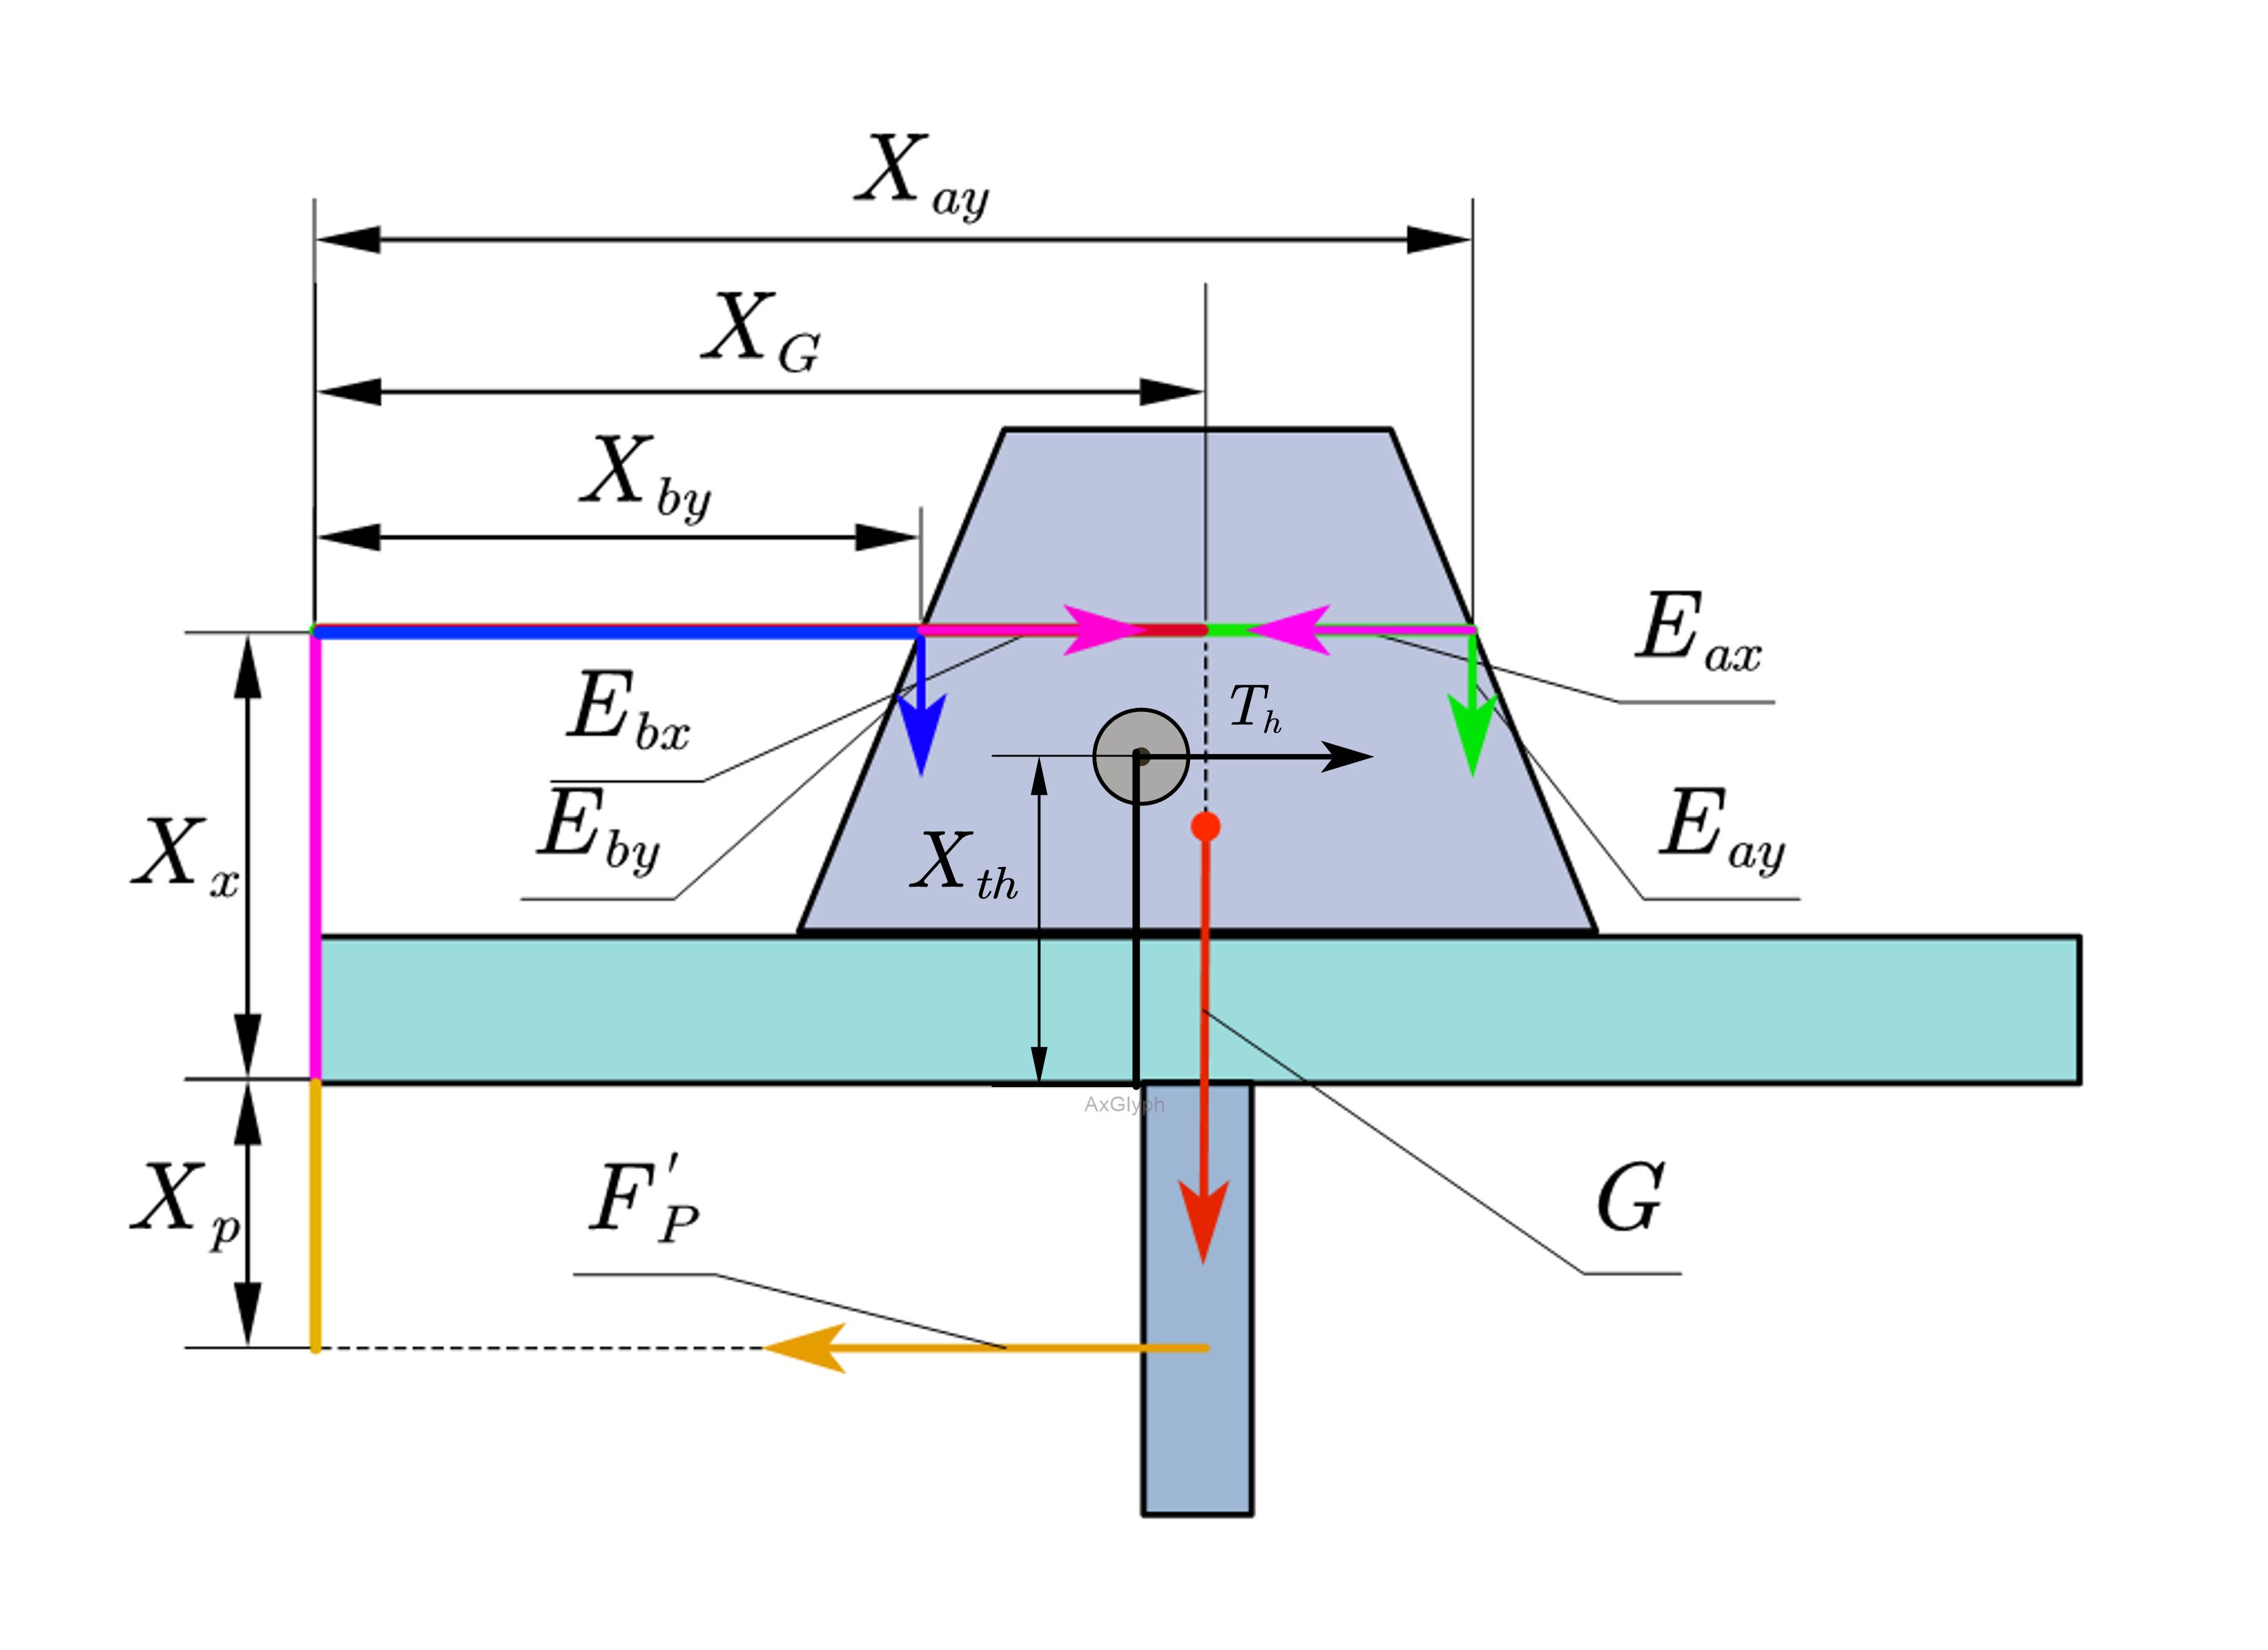
\includegraphics[width=0.5\textwidth]{拉筋.png}
        \caption{加入拉筋后力矩示意图}
        \label{fig:加入拉筋后力矩示意图}
    \end{figure}

图中清晰呈现了拉筋在扶壁式挡土墙中的力学作用机制,是模型二钢筋位置优化设计的核心可视化支撑。图中展示了拉筋的水平布置方式及其与墙面板、扶肋等构件的空间关系,直观反映了拉筋通过水平拉力\(T_h\)产生抗倾覆力矩的过程,该力矩以拉筋作用点到墙趾旋转中心的垂直距离为矩臂,直接抵消主动土压力的倾覆效应,同时其与土体的摩擦力可辅助提升抗滑移性能。
\par
图中隐含的拉筋位置参数\((x,y)\)是模型优化的关键变量,需严格满足多重约束条件。空间上,拉筋需位于墙体有效受力区域内,避免超出混凝土保护层范围;力学上,其拉力需控制在钢筋屈服强度与土体拔出阻力的限值内,确保工作在弹性阶段。这些约束通过图中虚线标注的安全边界与力的传递路径得以具象化,为非线性规划模型的约束条件设定提供了直观依据。
\par
该图直接支撑了模型二的优化结论,解释了拉筋最优位置的合理性。此位置下,拉筋力臂达到理论最优值,抗倾覆力矩与倾覆力矩形成最佳平衡,且锚固长度符合规范要求,既保证了结构安全,又避免了材料浪费。通过将抽象的力学公式转化为具象的空间-力关系,该图为拉筋优化设计的理论推导与结果验证提供了不可或缺的可视化支撑。
\subsection{模型求解}
综合以上模型,并结合模型一中所给约束条件,我们可以得到以下公式:
\begin{equation}
    \begin{array}{c} 
         max=k_w''=w_1k_s''+w_2k_t''\\[0.2cm]
            s.t.    
            \begin{aligned}
                \begin{cases}
                    k_s'' = \dfrac{[\gamma_1 V + (4L + 3t)E_{ay} + (4L + 3t)E_{by}]\mu + n\pi r L T_f + (4l + 3t)E_{bx}}{(4L + 3t)E_{ax}} \\
                    k_t'' = \dfrac{G_{ax}' X_G' + n\gamma_1 \pi r L T_f \left(B_L + \dfrac{b_2}{2}\right) + (4l + 3t)\left(E_{ay}X_{ay} + E_{by}X_{by}\right)}{(4L + 3t)\left(E_{ax} - E_{bx}\right)\dfrac{H}{3}} \\
                    + \dfrac{n\pi r \dfrac{D^2}{2}T_f + \dfrac{b_2}{2} + 2T_h(y + d_1)}{(4L + 3t)\left(E_{ax} - E_{bx}\right)\dfrac{H}{3}}\\
                    H\leq30 ,r\ge 0.3,L\leq\frac{H}{2}\\
                    t\in[\frac{L}{10},\frac{L}{4}],t\geq0.3 \\
                    b=k_{1}(B_{1}+B_{2}+b_{2})=k_{3}L \\
                    b_{1}\geq0.2 ,4L+3t\leq40 \\
                    B_{1}\in[\frac{H}{4},\frac{H}{2}],B_{2}\geq0.5 \\
                    B_{2}\in[\frac{H}{20},\frac{H}{5}],B_{2}\geq0.3 \\
                    b_{2}=b_{21}+b_{1}+b_{22} \frac{|tanx+y|}{\sqrt{tan\alpha^2+1} } \ge 0.04\\
                    tan\alpha=-\frac{H}{b_{21}},tan\beta=-\frac{H}{b_{22} }\\
                    \gamma_1=24,\gamma _2=18,\mu =0.6,\gamma _3=78.5\\\tau_t=0.92Mpa,\tau_t=30kMpa, V_{\text{max}} = \frac{q \cdot }{2}\\
                    D\in [\frac{H}{5}\frac{H}{2}],L_1\in [\frac{L}{5} ,\frac{L}{3} ],
                    M_{\text{max}} = \frac{q \cdot L^2}{8},\sigma_{\text{弯}} = \frac{M_{\text{max}}}{W}, \tau = \frac{V_{\text{max}}}{A_f}\\
                    q = \gamma \cdot h \cdot K_a,W = \frac{L \cdot b_1^2}{6}\\
                    p_{\text{max}} = \frac{G + E_{a,y}}{B} \left(1 + \frac{6e}{B}\right),
                    T_h\le min(\pi d_a\tau _t,F_p+f_\text{地} )\\
                    f_\text{地}=[\gamma _1V+\gamma _2V_j+(E_{a,y}+ E_{b,y})(4L+3t)]\mu ,\quad F_P=\pi rL_a\tau f\\
                     \frac{|-tan\beta \cdot x-y+tan\beta(b-\frac{H}{tan\beta}- \frac{H}{tan\alpha})|}{\sqrt{tan\beta^2+1} }\ge 0.04 \\
                    \alpha \cdot \frac{f_y}{f_t} \cdot d\le L_a\le \frac{4L+3t}{2}\\
                    x\in [0,-\frac{H}{tan\alpha } ],y\in [0.04, -tan\alpha ] \\
                    x\in [-\frac{H}{tan\alpha } ,b_1-\frac{H}{tan\alpha } ],y\in [0.04, H-0.04 ] \\
                    x\in [b_1-\frac{H}{tan\alpha } ,b_1-\frac{H}{tan\alpha }- \frac{H}{tan\beta }],y\in [0.04, -xtan\beta\\+tan\beta(b-\frac{H}{tan\beta}- \frac{H}{tan\alpha} ] 
                \end{cases}
            \end{aligned}
    \end{array}
\end{equation}

综合上述式子,我们可以得到:
    \begin{figure}[H]
        \centering
        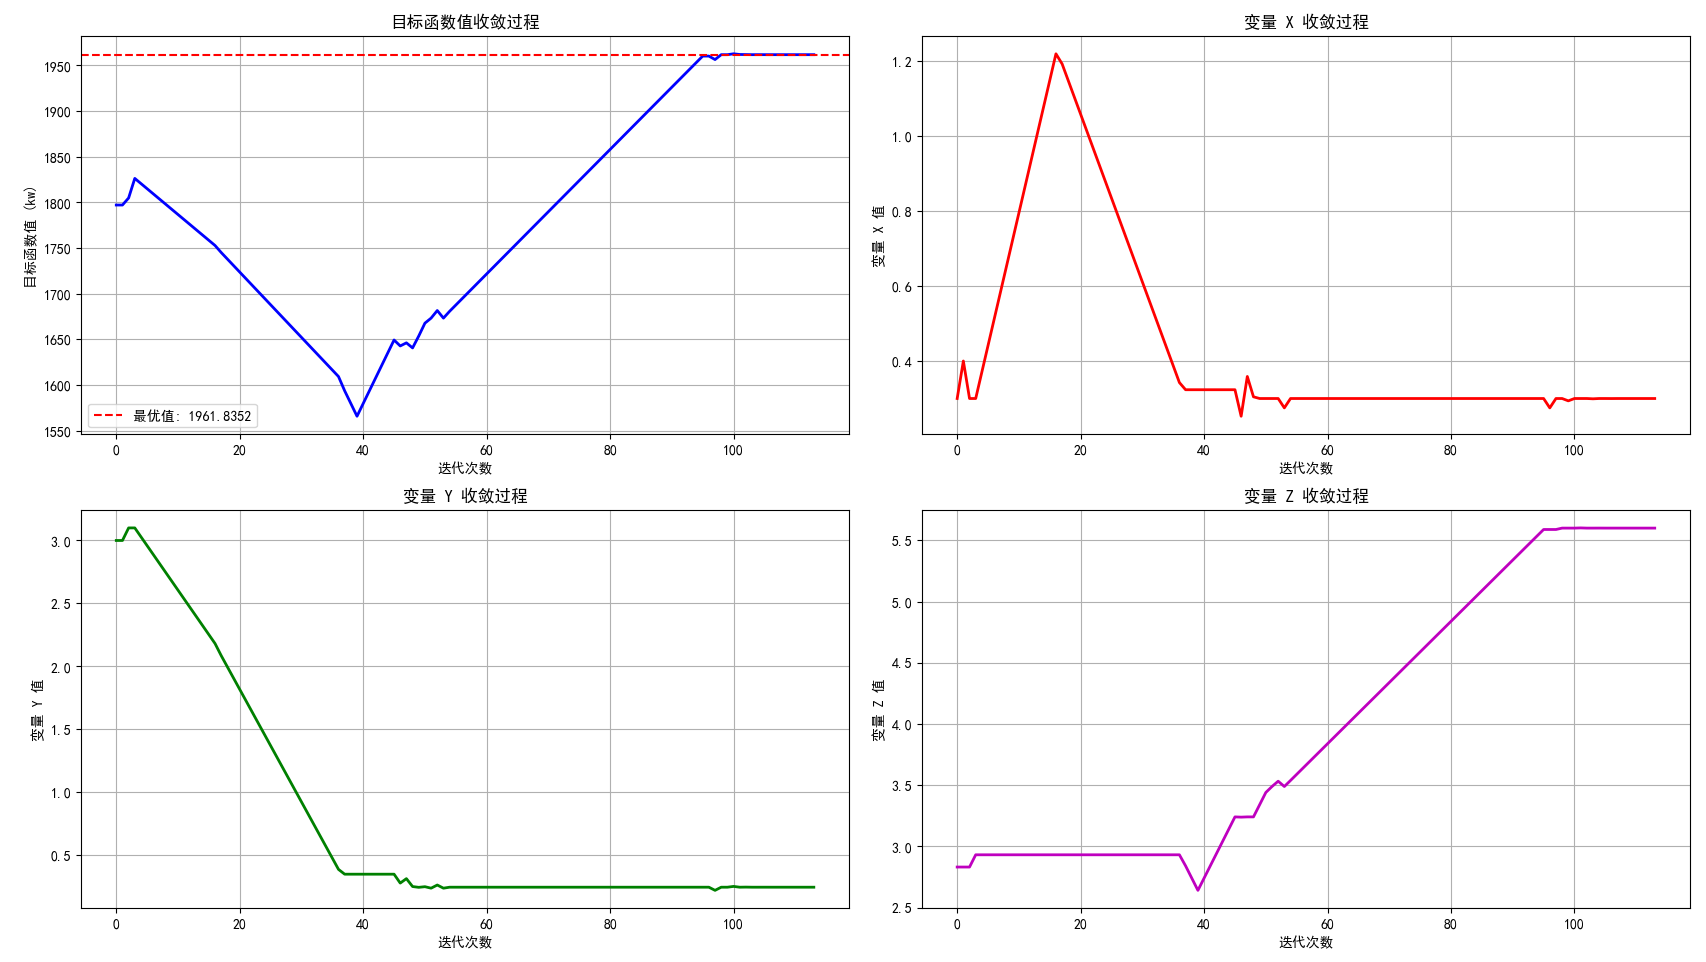
\includegraphics[width=0.8\textwidth]{迭代图.png}
        \caption{目标函数与拉筋位置优化过程}
        \label{fig:目标函数与拉筋位置优化过程}
    \end{figure}

从上图可知,当钢筋位置在($x$,$y$)=(0.3000,0.2434), 并且深度为 5.6000m,结果最优。


%%%%%%%%%%%%%%%%%%%%%%%%%%%%%%%%%%%%%%%%%%%%%%%%%%%%%%%%%%%%% 

\section{问题三的模型的建立和求解}
\subsection{基于非线性规划的泄水孔位置及数量稳定性最优化设计模型}
同问题二,我们在建立模型三时同样延用了上述基本模型,在此基础上添加了积水对挡土墙的影响,其中包括浮力对土体重度影响、降水对泄水孔层数影响、
泄水孔位置和墙厚水压力分布等众多因素。

\subsubsection{目标函数的建立}
同问题一,我们在建立模型时,主要考虑抗倾覆安全系数和抗滑移安全系数对总体稳定性影响。
因此,在上述模型上,我们针对泄水孔相关参数做了进一步扩充,可以得到:

    \begin{equation}
        \begin{aligned}
            \begin{cases}
                k_s''' = \dfrac{[\gamma_1 V + (4L + 3t)E_{ay} + (4L + 3t)E_{by}+(4L + 3t)P_{Wy}]\mu }{(4L + 3t)E_{ax}+P_{wy}} \\
                    + \frac{n\pi r L T_f + (4l + 3t)E_{bx}}{(4L + 3t)E_{ax}+P_{wy}}\\
                k_t'''= \dfrac{G_{ax}' X_G' +(P_{wy}+ n\gamma_1 \pi r L T_f) \left(B_L + \dfrac{b_2}{2}\right) }{(4L + 3t)\left(E_{ax} - E_{bx}\right)\dfrac{H}{3}+P_{wx}\frac{H}{3}} \\
                    +\dfrac{ (4l + 3t)\left(E_{ay}X_{ay} + E_{by}X_{by}\right)}{(4L + 3t)\left(E_{ax} - E_{bx}\right)\dfrac{H}{3}+P_{wx}\frac{H}{3}}\\
                    + \dfrac{n\pi r \dfrac{D^2}{2}T_f + \dfrac{b_2}{2} + 2T_h(y + d_1)}{(4L + 3t)\left(E_{ax} - E_{bx}\right)\dfrac{H}{3}+P_{wx}\frac{H}{3}}\\
            \end{cases}
            \end{aligned}
        \label{eq:stability}
    \end{equation}

将新的参数代入公式16中,可以得到目标函数:
    \begin{equation}
        k_w'''=w_1k_s'''+w_2k_t'''
    \end{equation}
    \par
其中,可以认为抗倾覆安全系数、抗滑移安全系数两者在本模型中同等重要,即$w_1=w_2=0.5$。
\subsubsection{浮力对土体重度影响}
墙后积水会使土体处于饱和状态,此时土体的有效重度$\gamma'$(扣除浮力后的重度)为:
    \begin{equation}
        \gamma'=\gamma_{sat}-\gamma_{w}
    \end{equation}

其中,$\gamma_{sat}$表示饱和土体重度,我们在这里采用的是砂性土,取值为20KN/$\mathrm{m^3}$。
并且在这里我们取$\gamma_{w}$为水的重度,取值为9.8KN/$\mathrm{m^3}$。
上述公式的意义为浮力抵消部分土体自重,导致作用于墙面板的主动土压力减小。

\subsubsection{主动土压力和被动土压力在浮力作用下的修正}
基于上述浮力的影响,我们修正了主动土压力和被动土压力,即:
    \begin{equation}
            \left\{
                \begin{aligned}
                    E_a=\frac{1}{2} \gamma_2'H^2K_a\\
                    E_b=\frac{1}{2} \gamma_2'H^2K_b
                \end{aligned}
            \right.
    \end{equation}

其中:$$\gamma_2'=\gamma_{sat}-\gamma_{w}=20-9.8=10.2\mathrm{KN/m^3}$$

\subsubsection{泄水孔层数设定}
泄水孔的层数由于其工程实用性、成本效益及结构安全性,应设定一个上限值。
在工程角度上,当泄水孔等数增加到一定程度后,额外增加层数对水压力的削减效果会显著减弱,此时继续增加层数无实际意义。
\par
在查阅相关文献后\upcite{YSGL202508007},我们将工程做了简化处理,即对墙高
$H$的挡土墙,层数常常满足:
    \begin{equation}
        n \leq \lceil H / 1.5 \rceil 
    \end{equation}
\par
在本题中,我们的取值为4,即间距为1.5m。


\subsubsection{水压力分布公式}
假设泄水孔将墙后水分段排出,每层孔对其控制范围内的水压力产生折减,墙后任意高度$z$
处的水压力为:
    \begin{equation}
        p_w(z) = \gamma_w \cdot \left[ z - \sum_{\substack{i=1 \\ h_i \leq z}}^{n} \lambda_i \cdot (z - h_i) \right]
    \end{equation}
    \par
其中,
$\lambda_i$表示单孔排水效率系数,反映第 $i$ 层孔的排水能力:
$$\lambda_i = \frac{a_i}{s_x \cdot s_y} \cdot C$$

\par 
其中 ,$a_i$表示第 $i$ 层单个泄水孔的横截面积;
 $s_x$ 和 $s_y$分别表示泄水孔在水平和垂直方向的间距;
$C$表示修正系数(通常取 $0.5 \sim 1$,取决于排水系统的通畅程度)。
$p_{w0}$表示无泄水孔时墙后最大静水压力:$$p_{w0} = \gamma_w H$$并且:
    \begin{itemize}
        \item 当 $z < h_1$(低于第一层泄水孔):无排水作用,水压力按线性分布 $p_w(z) = \gamma_w z$。
        \item 当 $h_i \leq z < h_{i+1}$(位于第 $i$ 层与第 $i+1$ 层孔之间):第 1 至第 $i$ 层孔共同作用,水压力因排水折减,折减幅度与 $\lambda_i$ 和孔位高度 $h_i$ 相关。
        \item 当 $z \geq h_n$(高于最上层泄水孔):所有泄水孔均起作用,水压力折减至最小。
    \end{itemize}
\par
因此我们可以得到总水压力与泄水孔位置的关系:
    \begin{equation}
        P_w = \int_{0}^{H} p_w(z) \, \mathrm{d} z
    \end{equation}
同时,为了后续表达,我们建立直角坐标系,如下图所示:
    \begin{figure}[H]
    \centering
    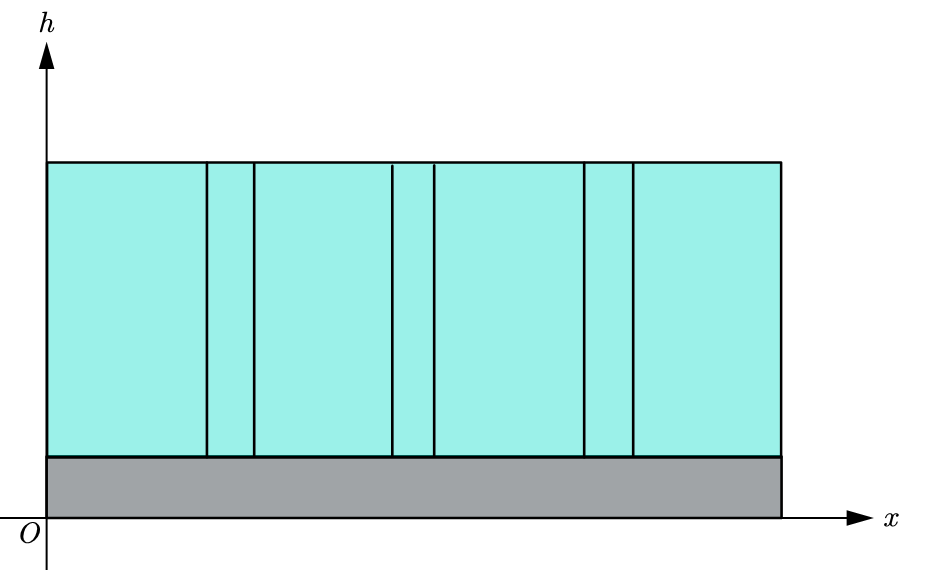
\includegraphics[width=0.5\textwidth]{坐标3.png}
    \caption{模型三坐标系图}
    \label{fig:模型三坐标系图}
    \end{figure}



\subsection{模型求解}
综合上述式子,结合之前的约束条件,我们可以得到以下公式:
$$max=k_w''' = w_1k_s''' + w_2k_t'''$$
\begin{equation}s.t.
    \begin{cases}
        \begin{aligned}
            k_s''' &= \dfrac{[\gamma_1 V + (4L + 3t)E_{ay} + (4L + 3t)E_{by}]\mu}{(4L + 3t)E_{ax} + P_{wy}} \\
            &+ \dfrac{n\pi r L T_f + (4l + 3t)(E_{bx}+P_{Wy}\mu)}{(4L + 3t)E_{ax} + P_{wy}}
        \end{aligned} \\[0.3cm]
        \begin{aligned}
            k_t''' &= \dfrac{G_{ax}' X_G' + (P_{wy} + n\gamma_1 \pi r L T_f) \left(B_L + \dfrac{b_2}{2}\right)}{(4L + 3t)\left(E_{ax} - E_{bx}\right)\dfrac{H}{3} + P_{wx}\dfrac{H}{3}} \\
            &+ \dfrac{(4l + 3t)\left(E_{ay}X_{ay} + E_{by}X_{by}\right)}{(4L + 3t)\left(E_{ax} - E_{bx}\right)\dfrac{H}{3} + P_{wx}\dfrac{H}{3}} \\
            &+ \dfrac{n\pi r \dfrac{D^2}{2}T_f + \dfrac{b_2}{2} + 2T_h(y + d_1)}{(4L + 3t)\left(E_{ax} - E_{bx}\right)\dfrac{H}{3} + P_{wx}\dfrac{H}{3}}
        \end{aligned} \\[0.3cm]
        P_{wx} = P_w\cos\left(\beta - \dfrac{\pi}{2}\right), \quad P_{wy} = P_w\sin\left(\beta - \dfrac{\pi}{2}\right) \\[0.2cm]
        E_a = \dfrac{1}{2} \gamma_2'H^2K_a, \quad E_b = \dfrac{1}{2} \gamma_2'H^2K_b \\[0.2cm]
        p_w(z) = \gamma_w \cdot \left[ z - \sum_{\substack{i=1 \\ h_i \leq z}}^{n} \lambda_i \cdot (z - h_i) \right] \\[0.2cm]
        P_w = \int_{0}^{H} p_w(z) \, \mathrm{d} z
    \end{cases}
\end{equation}

\begin{equation}s.t.
    \begin{cases}
        x_{ij} \in [(j-1)(L+t)+R, \, j(L+t)-t-R] \\[0.2cm]
        d_1 \le h_i \le H - R - \sin\beta \\[0.2cm]
        H \le 30, \quad r \ge 0.3, \quad L \le \dfrac{H}{2} \\[0.2cm]
        t \in \left[\dfrac{L}{10}, \dfrac{L}{4}\right], \quad t \ge 0.3 \\[0.2cm]
        b = k_{1}(B_{1} + B_{2} + b_{2}) = k_{3}L \\[0.2cm]
        b_{1} \ge 0.2, \quad 4L + 3t \le 40 \\[0.2cm]
        B_{1} \in \left[\dfrac{H}{4}, \dfrac{H}{2}\right], \quad B_{2} \ge 0.5 \\[0.2cm]
        B_{2} \in \left[\dfrac{H}{20}, \dfrac{H}{5}\right], \quad B_{2} \ge 0.3 \\[0.2cm]
        b_{2} = b_{21} + b_{1} + b_{22} \dfrac{| \tan x + y |}{\sqrt{\tan^2\alpha + 1}} \ge 0.04 \\[0.2cm]
        \tan\alpha = -\dfrac{H}{b_{21}}, \quad \tan\beta = -\dfrac{H}{b_{22}} \\[0.2cm]
        \gamma_1 = 24, \quad \gamma_2 = 18, \quad \mu = 0.6, \quad \gamma_3 = 78.5 \\[0.2cm]
        \tau_t = 0.92\,\text{MPa}, \quad \tau_t = 30\,\text{kPa}, \quad V_{\text{max}} = \dfrac{q \cdot}{2} \\[0.2cm]
        D \in \left[\dfrac{H}{5}, \dfrac{H}{2}\right], \quad L_1 \in \left[\dfrac{L}{5}, \dfrac{L}{3}\right] \\[0.2cm]
        M_{\text{max}} = \dfrac{q \cdot L^2}{8}, \quad \sigma_{\text{弯}} = \dfrac{M_{\text{max}}}{W}, \quad \tau = \dfrac{V_{\text{max}}}{A_f} \\[0.2cm]
        q = \gamma \cdot h \cdot K_a, \quad W = \dfrac{L \cdot b_1^2}{6} \\[0.2cm]
        p_{\text{max}} = \dfrac{G + E_{a,y}}{B} \left(1 + \dfrac{6e}{B}\right), \quad T_h \le \min(\pi d_a\tau_t, F_p + f_{\text{地}}) \\[0.2cm]
        f_{\text{地}} = [\gamma_1 V + \gamma_2 V_j + (E_{a,y} + E_{b,y})(4L + 3t)]\mu, \quad F_P = \pi r L_a \tau f
    \end{cases}
\end{equation}
\subsection{COBYLA 算法}
由于上述式子较为繁琐,约束多为非线性、非凸,且目标函数(稳定性指标)与设计变量(泄水孔坐标、半径、层数)的关系复杂,
难以用解析表达式完全刻画,因此我们在具体求解过程中采用了COBYLA 算法来简化运算。
\par
\textbf{Step1:定义设计变量}\par
将泄水孔的关键参数转化为优化变量向量\(x\):
\par
    \begin{equation}
        x = [r, \, h_1, \, x_{11}, \, x_{12}, \, ..., \, h_4, \, x_{41}, \, x_{42}, \, ...] 
    \end{equation}
\par
其中:\(r\)为泄水孔半径;\(h_i\)为第\(i\)层泄水孔的高度;\(x_{ij}\)为第\(i\)层第\(j\)个泄水孔的水平坐标。    

\par
\textbf{Step2:构建目标函数}\par
以稳定性指标\(k_w'''\)为优化目标:
\par
    \begin{equation}
        \min f(x) = -k_w'''(x)
    \end{equation}

\par

\textbf{Step3:定义约束条件}\par
将工程约束转化为不等式约束\(g(x) \leq 0\)。其中位置约束:泄水孔需位于挡土墙内部(如水平坐标\(x_{ij} \in [0.44, 9.95]\),高度\(h_i \in [1.25, 4.94]\));尺寸约束:半径\(r \geq 0.14\,\text{m}\),层间距\(\geq 1.5\,\text{m}\);
结构约束:泄水孔边缘距挡土墙边界至少0.04m(避免破坏墙体)。
\par
\textbf{Step4:算法迭代优化}\par
算法迭代大致上分成以下五种:初始点选择;线性近似;信赖域搜索;可行性检查;收敛判断。
我们首先设置初始解,再在当前迭代图中构建目标函数和线性模型,在信赖域中求解线性子问题,从而不断迭代,
在目标函数变化量小于阈值时,我们停止迭代。



\subsection{求解结果}
在模型求解释,我们通过python多次迭代,其中迭代图如下图所示:

    \begin{figure}[H]
        \centering
        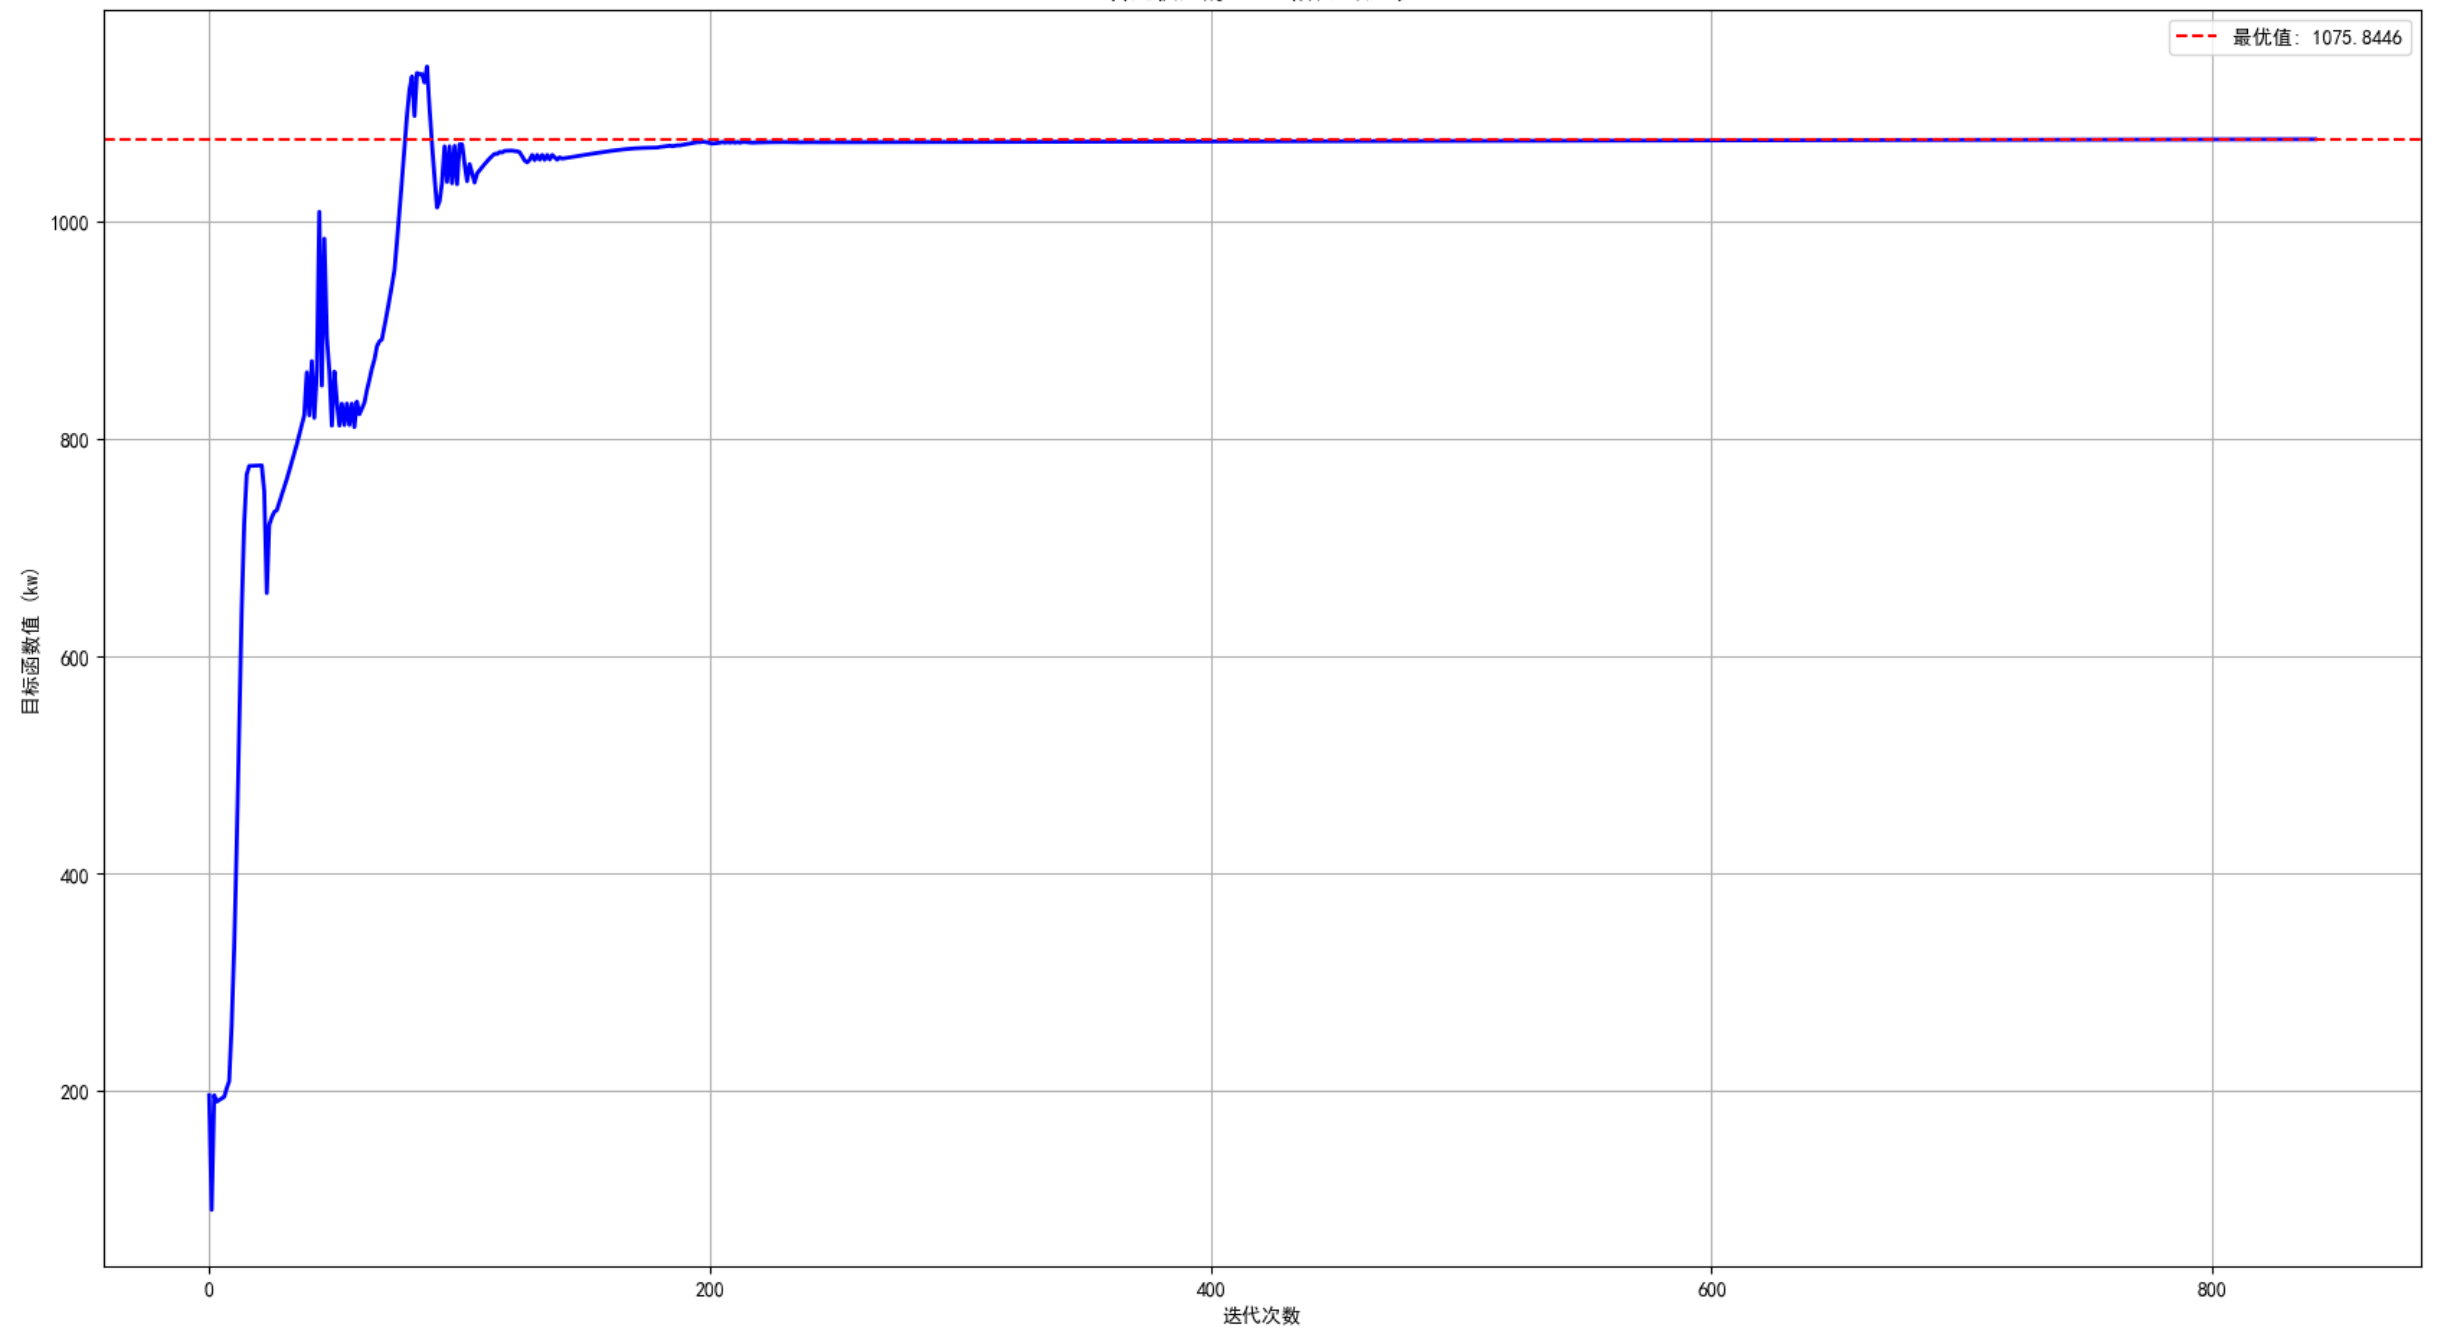
\includegraphics[width=0.5\textwidth]{迭代图2.png}
        \caption{目标函数收敛过程}
        \label{fig:单图}
    \end{figure}

最终求得泄水孔共有4层,每个半径为0.14米,
其坐标分别为0.44,1.25/1.94/3.44/4.94),(4.15,1.25/1.94/3.44/4.94),(7.05,
1.25/1.94/3.44/4.94),(9.95,1.25/1.94/3.44/4.94),单位为米。如下图所示:

    \begin{figure}[H]
        \centering
        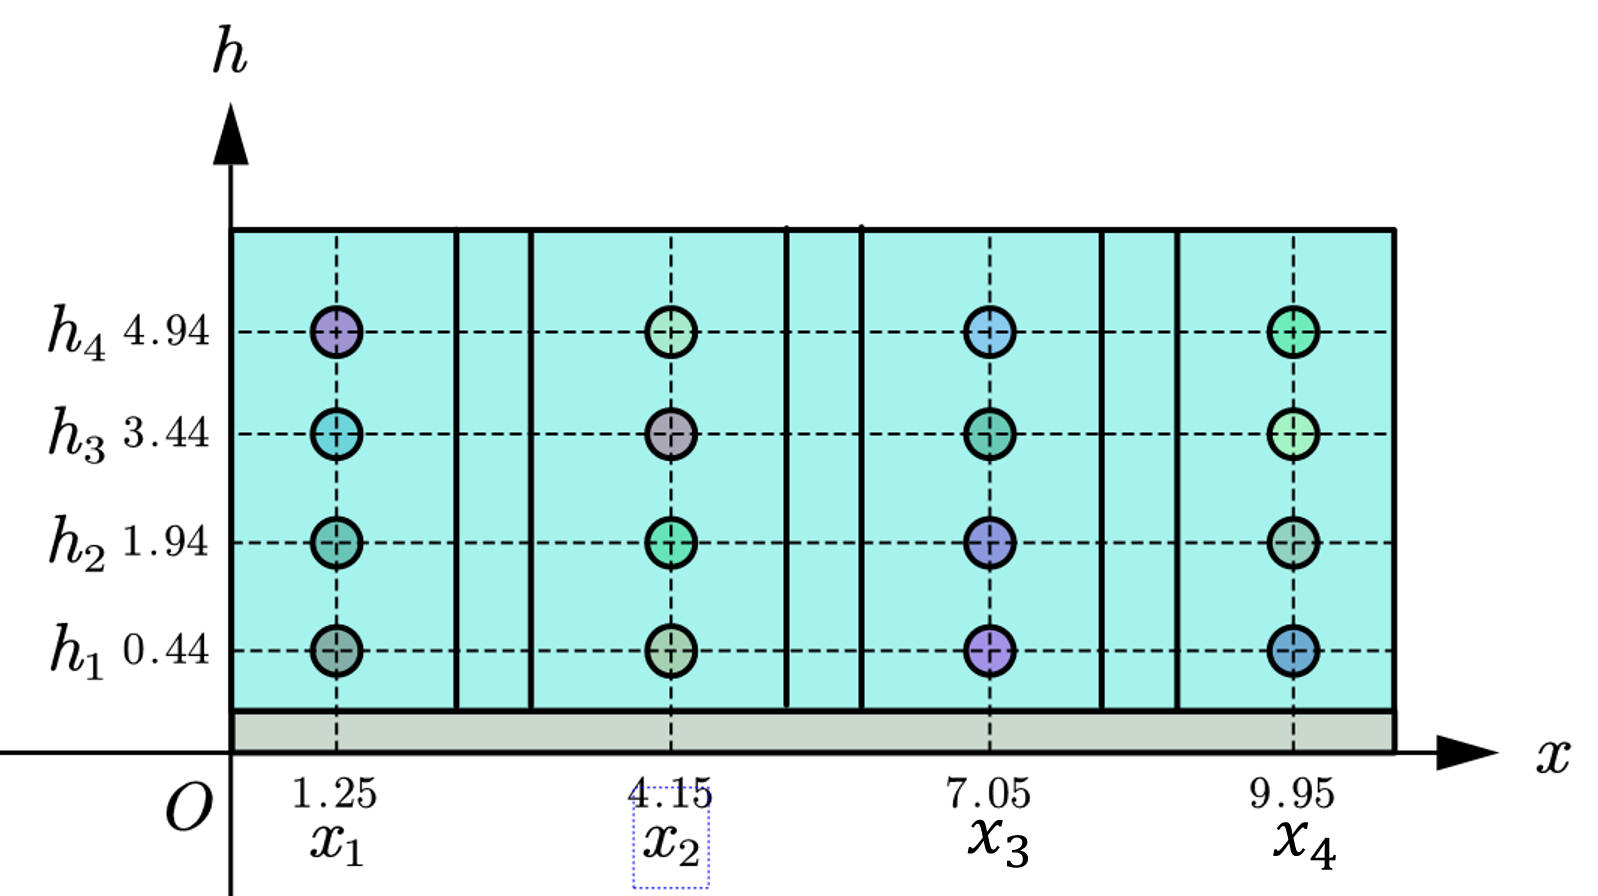
\includegraphics[width=0.5\textwidth]{坐标系3.png}
        \caption{泄水孔位置示意图}
        \label{fig:单图}
    \end{figure}


%%%%%%%%%%%%%%%%%%%%%%%%%%%%%%%%%%%%%%%%%%%%%%%%%%%%%%%%%%%%% 

% \section{问题四的模型的建立和求解}
% \subsection{模型建立}

% \subsection{模型求解}

% \textbf{Step1:} 

% \textbf{Step2:} 

% \textbf{Step3:} 

% \subsection{求解结果}

%%%%%%%%%%%%%%%%%%%%%%%%%%%%%%%%%%%%%%%%%%%%%%%%%%%%%%%%%%%%%

% \section{模型的分析与检验}

% \subsection{灵敏度分析}

% \subsection{误差分析}

%%%%%%%%%%%%%%%%%%%%%%%%%%%%%%%%%%%%%%%%%%%%%%%%%%%%%%%%%%%%%

\section{模型的评价}

\subsection{模型的优点}
\begin{itemize}[itemindent=2em]
\item 我们的模型具有较强的系统性和递进性,从模型一的单段无底桩到模型二的带底桩结构,
到模型三的考虑积水,逐步引入变量,逻辑清晰;
\item 我们核心模型基于库伦图压力理论计算土压力,结合多个评价指标,计算结果具有一定工程意义;
\item 在针对钢筋位置、泄水孔等参数设计时,我们采用非线性规划建立最优化模型,模型兼顾安全性和经济性。
\end{itemize}

\subsection{模型的缺点}
\begin{itemize}[itemindent=2em]
\item 由于题目所给条件较少,我们假设了较多条件,而实际工程中的复杂地形,很可能导致有相关压力计算的误差;
\item 模型仅为静态分析,并未考虑到山体滑坡的动态因素影响,难以反映长期的稳定性。
\end{itemize}

\subsection{模型的改进方向}
\begin{itemize}[itemindent=2em]
\item 模型下一步将引入动态分析,通过模拟雨水入渗过程,考虑土体抗剪强度的变化,从而预测工作性能;
\item 通过引入多个工程参数,考虑复杂地质情况,采用更精准的理论分析,减少假设误差。
\end{itemize}
%%%%%%%%%%%%%%%%%%%%%%%%%%%%%%%%%%%%%%%%%%%%%%%%%%%%%%%%%%%%%
%% 参考文献
\nocite{*}
\bibliographystyle{gbt7714-numerical}  % 引用格式
\bibliography{ref.bib}  % bib源

\newpage
%%%%%%%%%%%%%%%%%%%%%%%%%%%%%%%%%%%%%%%%%%%%%%%%%%%%%%%%%%%%%
%% 附录
\begin{appendices}
\section{文件列表}
\begin{table}[H]
\centering
\begin{tabularx}{\textwidth}{LL}
\toprule
文件名   & 功能描述 \\
\midrule
q1.py & 问题一程序代码 \\
q2.py & 问题二程序代码 \\
q3.py & 问题三程序代码 \\
\bottomrule
\end{tabularx}
\label{tab:文件列表}
\end{table}

\section{代码}
\noindent q1.py
\lstinputlisting[language=matlab]{code/q1.py}
q2.py
\lstinputlisting[language=python]{code/q2.py}
q3.py
\lstinputlisting[language=c]{code/q3.py}
\end{appendices}
\end{document}


%%%%%双图模板%%%%%%
\begin{figure}
\centering
\subcaptionbox{炉温曲线示意图\label{fig:双图a}}
{\includegraphics[width=.4\textwidth]{炉温曲线示意图.png}}
\subcaptionbox{问题1炉温曲线\label{fig:双图b}}
{\includegraphics[width=.4\textwidth]{问题1炉温曲线.png}}
\caption{双图}\label{fig:双图}
\end{figure} 
%%%%%双图模板%%%%%%